%\documentclass[paper]{geophysics}
\documentclass[paper, twocolumn]{geophysics} %revised paper manuscript

\usepackage[pdftex]{graphicx}
\graphicspath{{../Figures/300dpi/}}

%\usepackage{subcaption}
%\usepackage{setspace}
%% Math or theory people may want to include the handy AMS macros
\usepackage{amssymb}
\usepackage{float}
\usepackage[fleqn]{amsmath}
\usepackage{amsfonts}
\usepackage{wrapfig}
\usepackage{hyperref}
\usepackage{url}

%\usepackage{algorithm}
%\usepackage{algorithmicx}

% Somehow \nl means \newline here and is in conflict with algorithm2e
%\let\nl\undefined
%\usepackage[linesnumbered, algoruled, lined, commentsnumbered,algo2e]{algorithm2e} % [linesnumbered, algoruled, lined, commentsnumbered,
%\usepackage{algpseudocode}

% An example of defining macros
\newcommand{\rs}[1]{\mathstrut\mbox{\scriptsize\rm #1}}
\newcommand{\rr}[1]{\mbox{\rm #1}}
%\usepackage[utf8]{inputenc}

% \newcommand{\mathbf}[1]{
%   \hbox{\mathversion{bold}$#1$}}
\newcommand{\rmn}[1] {{\mathrm #1}}
\newcommand{\itl}[1] {{\mathit #1}}
\newcommand{\bld}[1] {{\mathbf #1}}


\begin{document}

\title{Joint inversion of potential fields data over the DO-$27$ kimberlite pipe using a Gaussian mixture model prior\footnotemark[1]}

% \renewcommand{\thefootnote}{\fnsymbol{footnote}}

% \ms{10.1190/int-2019-0283.1} % manuscript number

% \address{\\
% \footnotemark[1] DOI: \url{https://doi.org/10.1190/int-2019-0283.1} \\
% \footnotemark[2] Geophysical Inversion Facility,
% \footnotemark[3] Mira Geoscience
% }
% \author{Thibaut Astic\footnotemark[2], Dominique Fournier\footnotemark[3],
% and Douglas W. Oldenburg\footnotemark[2]}

% \footer{\url{https://doi.org/10.1190/int-2019-0283.1}}
% \lefthead{Astic, Fournier \& Oldenburg}
% \righthead{Petrophysically Coupled Joint Inversion}

% \maketitle

%\let\leqslant=\leq
%\newtheorem{theorem}{Theorem}[section]


\begin{abstract}
\begin{footnotesize}
We carry out petrophysically and geologically guided inversions (PGI) to jointly invert airborne and ground-based gravity data and airborne magnetic data to recover a quasi-geologic model of the DO-$27$ kimberlite pipe in the Tli Kwi Cho (TKC) cluster. DO-$27$ is composed of three main kimberlite rock types in contact with each other and embedded in a granitic host rock covered by a thin layer of glacial till. The pyroclastic kimberlite (PK), which is diamondiferous, and the volcanoclastic kimberlite (VK) have anomalously low density, due to their high porosity, and weak magnetic susceptibility. They are indistinguishable from each other based upon their potential field responses. The hypabyssal kimberlite (HK), which is not diamondiferous, has been identified as highly magnetic and remanent. Quantitative petrophysical signatures for each rock unit are obtained from sample measurements, such as the increasing density of the PK/VK unit with depth and the remanent magnetization of the HK unit, and represented as a Gaussian Mixture Model (GMM). This GMM guides the PGI towards generating a three dimensional quasi-geologic model with physical properties that both satisfies the geophysical datasets and the petrophysical signatures. Density and magnetization models recovered individually yield volumes that have physical properties combinations that do not conform to any known petrophysical characteristics of the rocks in the area. A multi-physics PGI addresses this problem by using the GMM as a coupling term but puts a volume of PK/VK unit at a location that is incompatible with geologic information from drillholes. To conform with that geological knowledge, a fourth unit is introduced, PK-minor, which is petrophysically and geographically distinct from the main PK/VK unit. This inversion produces a quasi-geologic model that presents good structural locations of the diamondiferous PK unit and can be used to provide a resource estimate or decide the locations of future drillholes.
\end{footnotesize}
\end{abstract}

%______________________________________________________________________________
\section{Introduction and geological setting}

%\plot{Figure1.png}{width=\columnwidth}{Topography map (gray contours and shaded background) and hydrography (blue) at the DO-$27$ kimberlite pipe in the Northwest Territories, Canada (location in inset). The area of interest is represented as a dashed box. Outline of the PK/VK (dashed) and HK (solid) kimberlite facies present in the pipe are extracted from the geologic model at $285$ m of elevation are overlaid on the map. DO-$18$ is visible at the northern boundary of the map. Geographic projection: UTM 12N, NAD27.}

\begin{figure}
\centering
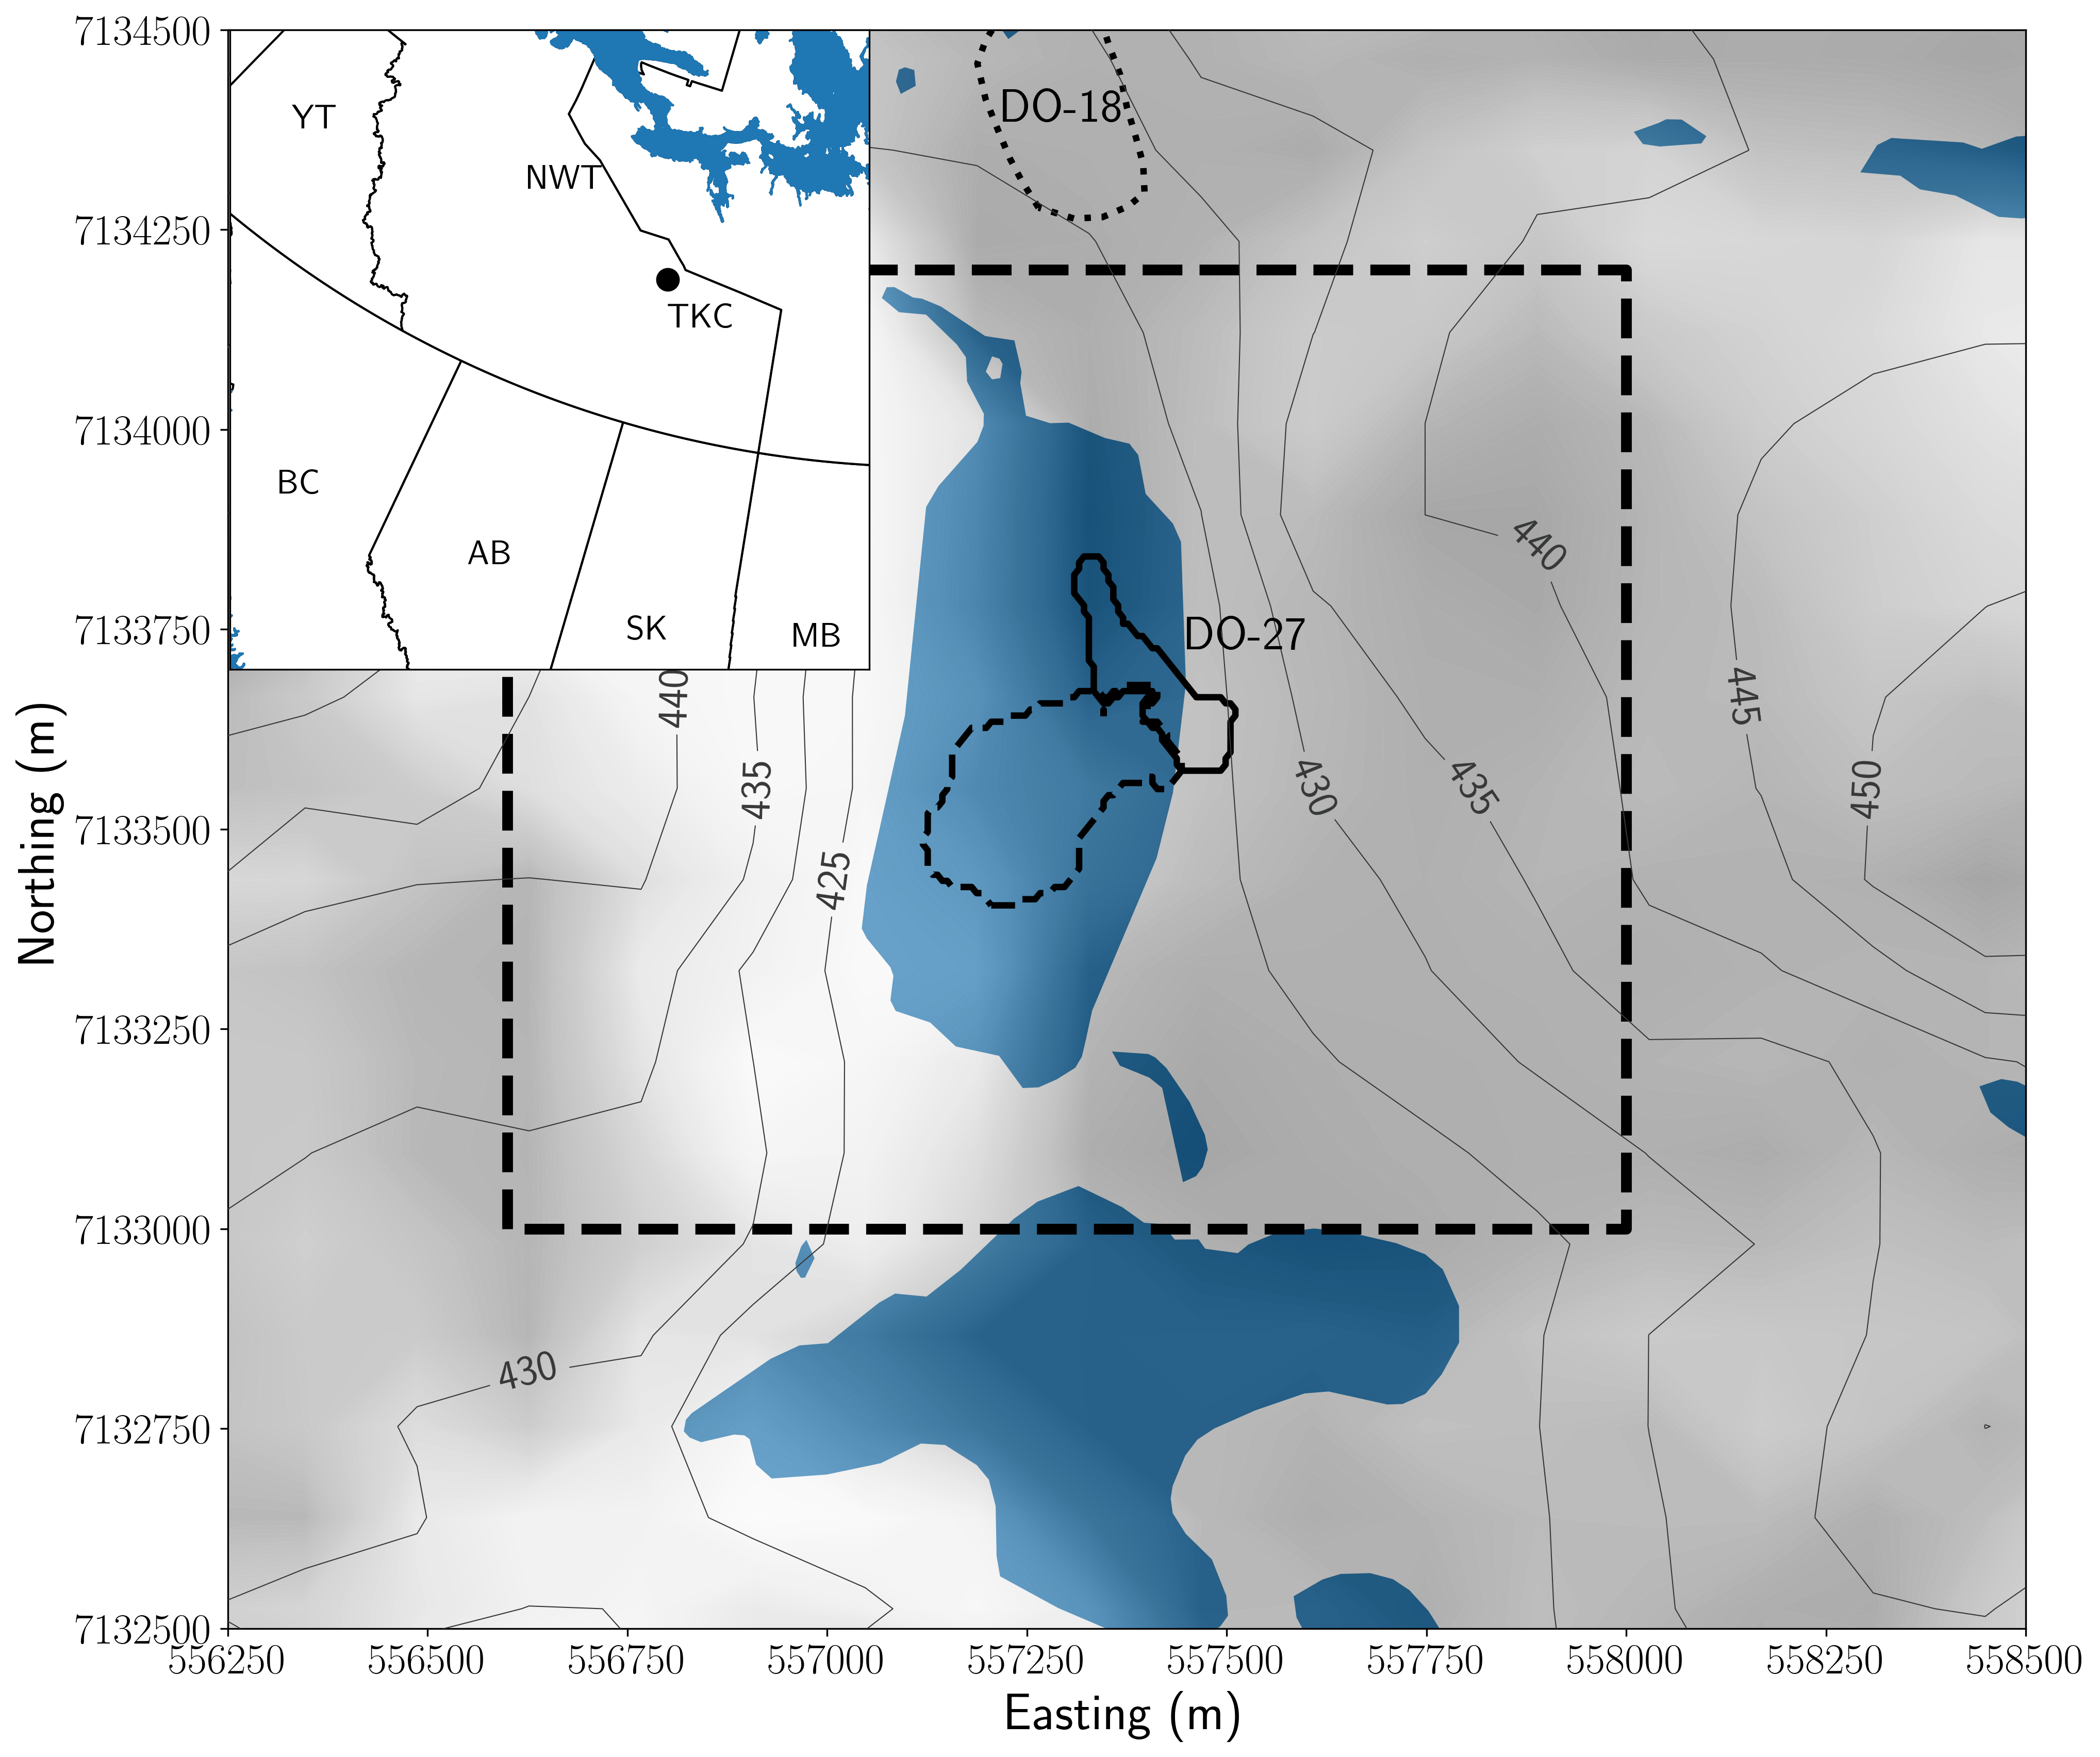
\includegraphics[width=\columnwidth]{Figures/300dpi/Figure1.png}
\caption{Topography map (gray contours and shaded background) and hydrography (blue) at the DO-$27$ kimberlite pipe in the Northwest Territories, Canada (location in inset). The area of interest is represented as a dashed box. Outline of the PK/VK (dashed) and HK (solid) kimberlite facies present in the pipe are extracted from the geologic model at $285$ m of elevation are overlaid on the map. DO-$18$ is visible at the northern boundary of the map. Geographic projection: UTM 12N, NAD27.}
\label{fig:Figure1.png}
\end{figure}

The DO-$27$ kimberlite pipe is located in the kimberlite-rich Lac De Gras region, Northwest Territories, Canada (Figure \ref{fig:Figure1.png}). It was first discovered in 1992, following the discovery of the Ekati kimberlite field in September 1991 \citep{DiamondsInCanada}, thanks to an airborne frequency-domain electromagnetic survey (DIGHEM). Two distinct anomalies were identified, which were initially thought to be part of a single large complex. After multiple revisions of the conceptual geologic model \citep{HARDER2009}, it is now believed that there are two main pipes, designated DO-$18$ and DO-$27$, with distinct rock types. Kimberlite pipes are potentially diamondiferous, and the assessment of their economic potential requires an understanding of their geologic structures.

%While an initially optimistic resource estimate warranted further exploration work, the uncommon geology of the deposit necessitated multiple revisions of the conceptual model, each time lowering its inferred resource \citep{HARDER2009}. It is made up of two main pipes, designated DO-$18$ and DO-$27$, with distinct rock types. These are potentially diamondiferous, but the assessment of their economic potential requires an understanding of the geology of the pipes.

Several types of kimberlite facies can reside inside the same pipe. A schematic representation of the architecture of a typical Lac de Gras pipe is shown in Figure \ref{fig:Figure2.png}a. The various kimberlite facies are classified based on their genesis \citep{KimberliteModel0,KimberliteModel1}. At DO-$27$, there are three main facies, embedded in a granitic host rock, that play a role in the potential field responses. The first is a hypabyssal (HK) kimberlite, which is an intrusive igneous rock often found at the base of the pipe (Figure \ref{fig:Figure2.png}). The second is a volcanoclastic kimberlite (VK), which is an extrusive igneous rock with high porosity, that is typically found above the HK unit. The last facies is a pyroclastic kimberlite (PK), which is the diamondiferous unit at DO-$27$. It shares many characteristics with VK as both formed during extrusion events accompanied by an explosion. Glaciers eroded the top of the pipes, allowing the formation of lakes, and deposited a thin layer of till \citep{Dyke,Doyle}.

The geologic model of the DO-$27$ pipe, built from several drilling campaigns, is presented in Figure \ref{fig:Figure2.png}b. The geometry of DO-$27$ diverges significantly from the standard kimberlite model with a sheet-like hypabyssal unit present near the surface. \citet{HARDER2009} concluded that DO-$27$ was formed in several successive volcanic phases with the HK unit pre-dating the VK intrusion \citep{Doyle}. This VK intrusion was later disturbed by another volcanic event, with the PK unit infilling the pipe. Several minor occurrences of kimberlite units have been observed close to the surface, that have been identified as PK facies. As discussed in \citet{TKCpaper}, the density and magnetic characteristics of the different units are as follows: (a) the PK and VK units have low density and are weakly magnetic susceptible. They are indistinguishable from each other in potential field surveys, and we thus refer to them as a PK/VK unit; (b) the HK unit has a density that is close to the granitic host rock, but it has a high magnetic susceptibility and is remanently magnetized; (c) the thin horizontal layer of glacial till, that only plays a minor role from a potential field standpoint, and granitic host rock are regrouped under the term "background".

%The expected qualitative physical properties signature for each unit present at DO-$27$, used for previous studies in the area, are presented in Table \ref{tbl:pp}. Because of their similarities, the PK and VK kimberlites are indistinguishable from each other based on their gravity and magnetic responses. We thus refer to those two units as a single entity PK/VK. For the same reason, we regroup the granitic host rock and the glacial tills as "background".

%\plot{Figure2.png}{width=\columnwidth}{(a) Lac De Gras kimberlite pipe conceptual model (modified from \citet{TKCpaper}). HK: Hypabyssal Kimberlite facies; VK: Volcanoclastic Kimberlite facies; PK: Pyroclastic kimberlite facies; (b) Current geological representation of the DO-$27$ pipe based on drillholes. The same color convention for the rock units is used for panels (a) and (b) and throughout the paper.}

\begin{figure*}
\centering
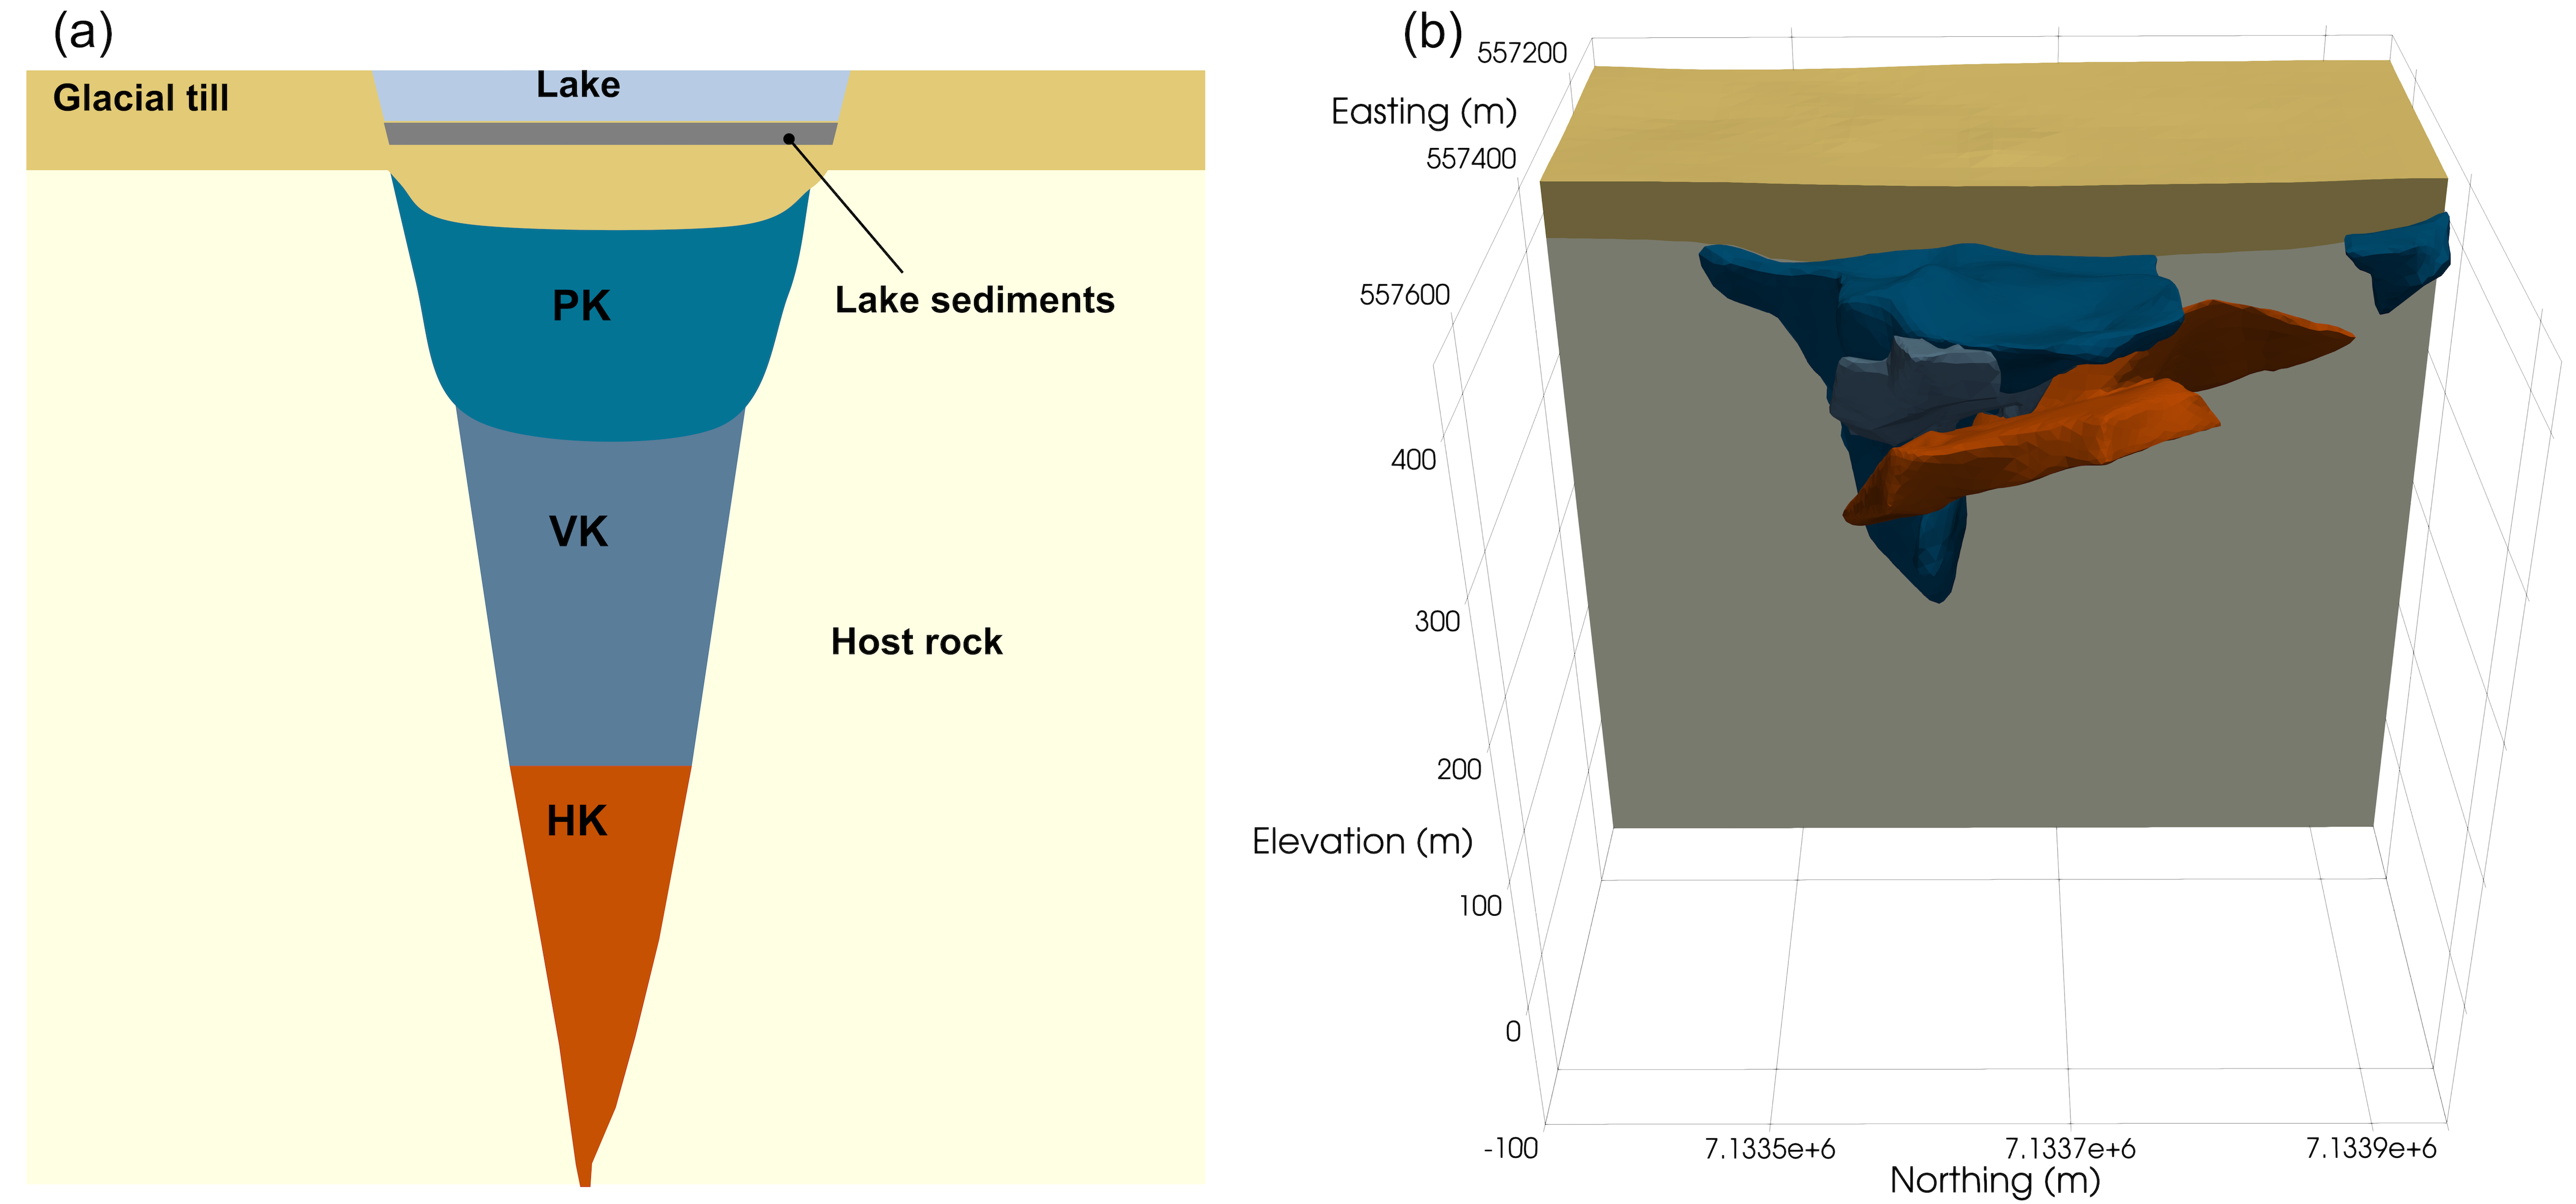
\includegraphics[width=\textwidth]{Figures/300dpi/Figure2.png}
\caption{(a) Lac De Gras kimberlite pipe conceptual model (modified from \citet{TKCpaper}). HK: Hypabyssal Kimberlite facies; VK: Volcanoclastic Kimberlite facies; PK: Pyroclastic kimberlite facies; (b) Current geological representation of the DO-$27$ pipe based on drillholes. The same color convention for the rock units is used for panels (a) and (b) and throughout the paper.}
\label{fig:Figure2.png}
\end{figure*}

%\tabl{pp}{Qualitative physical properties expected in the Lac de Gras region.}{
%\begin{center}
%\scalebox{0.9}{
%\begin{tabular}{|c|c|c|}
%\hline
%Rock type & Density & Susceptibility \\
%\hline
%Glacial till & moderate & none \\
%Host rock & moderate & none \\
%PK & low & low-moderate \\
%VK & low & low-moderate \\
%HK & low-moderate & high \\
%\hline
%\end{tabular}}
%\end{center}
%}

%Kimberlites typically present a geophysical signature comprised of a strong magnetic response, often with a remanent component, and a low density.
%little geophysical analysis was done at the time of the discovery of the DO-$18$ and DO-$27$ complex, partly due to the limited access to modeling software at the time. Since then, several studies have been dedicated to the geophysical datasets.

Geophysics plays an important role in kimberlite exploration \citep{Macnae,Keating,Power}, and much work has been done over the DO-$27$ and DO-$18$ kimberlite pipes. \citet{JansenEtAl2004} presented an overview of the exploration geophysical surveys acquired before 2000. \citet{TKCpaper} performed smooth inversions of individual potential field datasets. Their interpretation of the physical property models defined the overall shape of the DO-$27$ and DO-$18$ pipes. Their analysis provided a valuable start in distinguishing between the PK/VK and the HK units. \citet{TKCEM} focused on the inversion and interpretation of the electromagnetic surveys. They were able to distinguish the top of the pipe from the lake-bottom sediments and till layer. Finally, \citet{TKCIP} extracted Induced Polarization information from airborne electromagnetic surveys to distinguish between adjacent kimberlites based on their clay mineral content. They subsequently built a geologic model using a post-inversion classification. The inputs to the classification were density, magnetic susceptibility, electrical conductivity, and chargeability obtained from the individual smooth inversions.

The use of post-inversion classification to infer geologic information has been widely used, for example in \citet{OldenburgMilligan1997,PostInversionClustering1,PostInversionClustering0,PostInversionClustering2,PostInversionClustering3} and \citet{Melo2017}. However, there are challenges in using this methodology. Geophysical inversion generally produces a smooth image of the Earth, and the details are dependent upon parameters in the inversion. Building a geologic model from these inversions also requires specifying thresholds and criteria to discriminate between rock units; these are subjective choices and need expert knowledge that can make post-inversion classification challenging for problems such as resource estimation, which for DO-$27$ is linked to the volume of the PK/VK unit. Rather than generate a quasi-geologic model from a post-inversion classification \citep{QuasiGeologicalModel}, our goal is to carry out a single inversion that integrates potential fields data with petrophysical and geological information. We use a joint inversion framework \citep{ggz389,AsticJoint} for petrophysically and geologically guided inversion (PGI). It produces physical property models that fit both geophysical and petrophysical data, which allows the inversion to build a quasi-geologic model. In this study, we jointly invert potential fields data from a ground gravity survey, an airborne gravity gradiometry (Falcon) survey \citep{FalconPaper}, and an airborne magnetic survey (acquired during a VTEM survey \citep{VTEM}). We use the petrophysical signatures of the background, PK/VK, and HK rock units as a coupling term. This coupling term links density, the three components of the magnetization of the rocks, and the elevation to account for variations of the density signature of the PK/VK unit with depth. The petrophysical data are represented as a Gaussian Mixture Model (GMM) \citep{ExpectationMaximization, Murphy2012}. This GMM is used to generate a misfit function that quantifies how well the inversion fits the petrophysical signatures. A successful inversion simultaneously achieves acceptable fits of the geophysical and petrophysical data.

This study is segmented into five parts. First, we introduce the geophysical datasets and our data processing steps. We then summarize our PGI methodology for representing petrophysical and geological information and how to include it in an inversion. Next, we design the GMM from the available petrophysical data by identifying the physical properties characteristics of each rock unit. Our first inversion with the PGI approach focuses on recovering density from the two gravity surveys. We jointly invert ground gravity and Falcon data to recover a density model that is consistent with the PK/VK density increase with depth. We then invert the magnetic data from the VTEM survey. To recover a magnetization model consistent with the high remanence of the HK unit, we use a Magnetic Vector Inversion (MVI). We show that combining these density and magnetic vector models yields volumes with erroneous combinations of physical properties and uncertainties about the extent of the HK and PK/VK units.
We follow up with a fully integrated multi-physics inversion of the potential field datasets by inverting all three geophysical surveys together with the signature of all three rock units (background, PK/VK, and HK). This model is a significant improvement over what is obtained from post-inversion classifications. The delineation of the diamondiferous PK/VK unit over the central part of the DO-27 pipe is in good agreement with the outline drawn from drillholes. The model, however, disagrees with drillhole information north of the DO-$27$ pipe. To address this, we add to our inversion geological information from drillholes and an extra rock unit to represent minor near-surface occurrences of PK facies. The final quasi-geologic model obtained with our PGI approach resolves the geologic conflicts and allows us to estimate the volume of the PK/VK unit, which is the potential diamondiferous resource at DO-$27$.

%A first model without localized geological information shows a clear delineation of the two kimberlite bodies. However, some features disagree with available drillhole information. We thus finally include geological a priori information from drillholes, along with an additional rock unit to represent minor near-surface occurrences of PK facies, to our joint inversion to help the recovery of the desired geological features. This final quasi-geologic model obtained from inversion allows us to estimate the volume of the PK/VK unit, which is the potential diamondiferous resource.

%______________________________________________________________________________
\section{Geophysical datasets}

%\plot{Figure3.png}{width=\textwidth}{Four potential field datasets, collected over the DO-$27$ pipe, that are used in this study (after regional removal). (a) Airborne VTEM total field magnetic survey; (b) Ground gravity survey; (c) $G_{xy}$ component of the airborne Falcon gravity gradiometry survey; (d) $G_{uv}$ component of the airborne Falcon gravity gradiometry survey.}

\begin{figure*}[!ht]%*
\centering
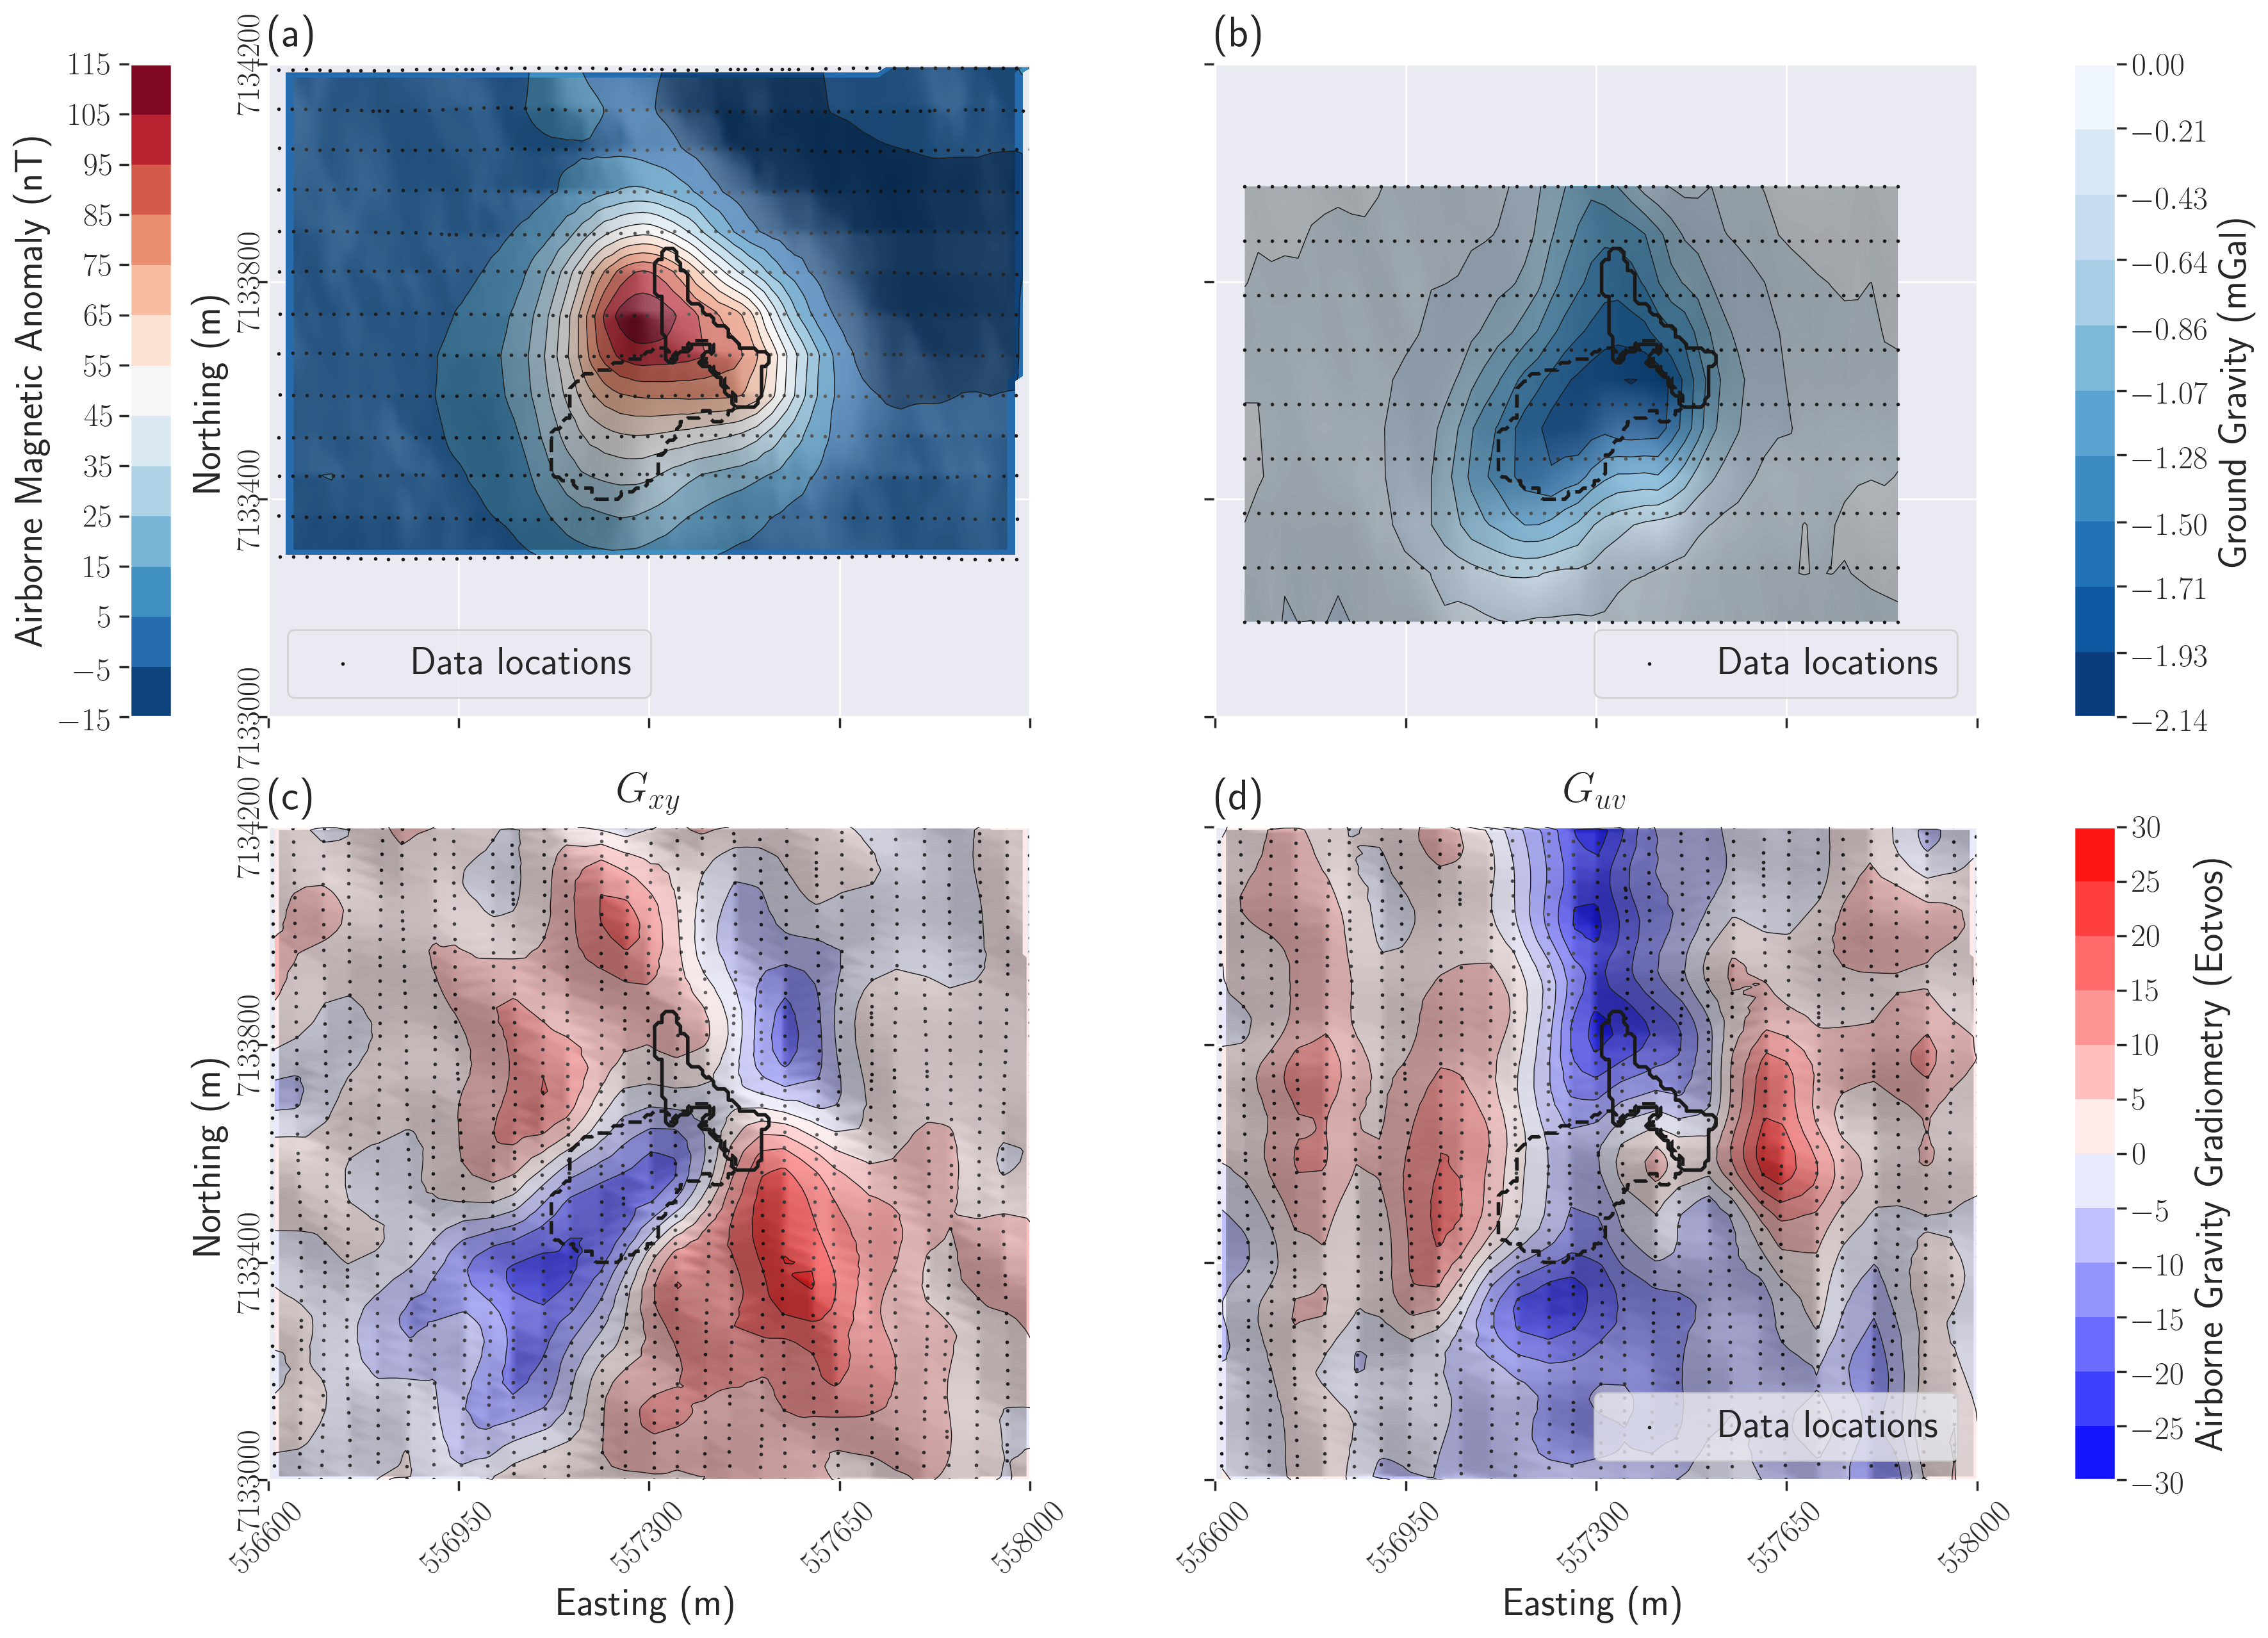
\includegraphics[width=\textwidth]{Figures/300dpi/Figure3.png}
\caption{Four potential field datasets, collected over the DO-$27$ pipe, that are used in this study (after regional removal). (a) Airborne VTEM total field magnetic survey; (b) Ground gravity survey; (c) $G_{xy}$ component of the airborne Falcon gravity gradiometry survey; (d) $G_{uv}$ component of the airborne Falcon gravity gradiometry survey.}
\label{fig:Figure3.png}
\end{figure*}%*

%In this section, we present the various geophysical datasets acquired at DO-$27$ that we use in this study.

\subsection{Ground gravity}

Ground gravity data were acquired, on the ice, over DO-$27$ in the spring of 1994. The survey is composed of 441 stations with a $25$ m spacing along East-West lines $100$ m apart. Gravity data were processed by the contractor and provided as the complete Bouguer anomaly.

In preparation for the inversion, we upward continued the data by $6.25$ m so that the data are half a cell width above the surface. This is done to minimize the effects of potential small scale heterogeneities inside a subsurface cell that is mathematically modeled as a volume with homogeneous density \citep{Li1996}. A low-frequency signal was seen in our early inversions that manifested as density contrasts in the padding cells. While this low-frequency signal can be absorbed this way, we chose to remove a linear trend from the data to focus the inversion on the local anomalies. We used a robust Cauchy loss function for the linear regression, which is less affected by outliers than a least-squares estimation \citep{CauchyNorm}. The processed dataset is shown in Figure \ref{fig:Figure3.png}b.
%To ameliorate harmful effects from local inhomogeneities

A clear negative anomaly of $-2.14$ mGal, associated with the DO-$27$ kimberlite pipe, is visible. A northern extension was first interpreted as a connexion between the DO-18 and the DO-$27$ kimberlite pipes. The current understanding is that it is due to several minor near-surface kimberlite dikes and sills \citep{Doyle}.

In the inversion, we assign a uniform unbiased Gaussian noise level with a standard deviation of $0.045$ mGal; this is identical to what is used in \citet{TKCpaper}.

\subsection{Falcon airborne gravity gradiometry}

An airborne Falcon gravity gradiometry survey was flown in 2001 over the property. Over the area of interest, the survey flew $29$ North-South flight lines spaced $50$ m apart at an average $53$ m ground clearance. We down-sampled the data along the lines to one measurement every $25$ m to yield approximately one data point per surface cell in our mesh. This ensures there is no signal in the data with a smaller wavelength than can be modeled by the mesh (Figure \ref{fig:Figure3.png}c and \ref{fig:Figure3.png}d).

At each station, two combinations of the gravity gradiometry tensor \citep{GG} are measured by the Falcon system \citep{FalconPaper}. The first component is simply $G_{xy}$. The second measurement is a linear combination of two components of the tensor: $G_{uv} = (G_{yy}-G_{xx}) / 2$. We invert directly for those two measurements. The data were processed by the contractor with an equivalent source transformation using a $2.67 \text{ g/cm}^3$ background density.

In the inversion, we assign a uniform unbiased Gaussian noise level with a standard deviation of $5$ eotvos for both $G_{xy}$ and $G_{uv}$ components; this is identical to the one used in \citet{TKCpaper}.

\subsection{Airborne magnetic survey}


\begin{figure*}
\centering
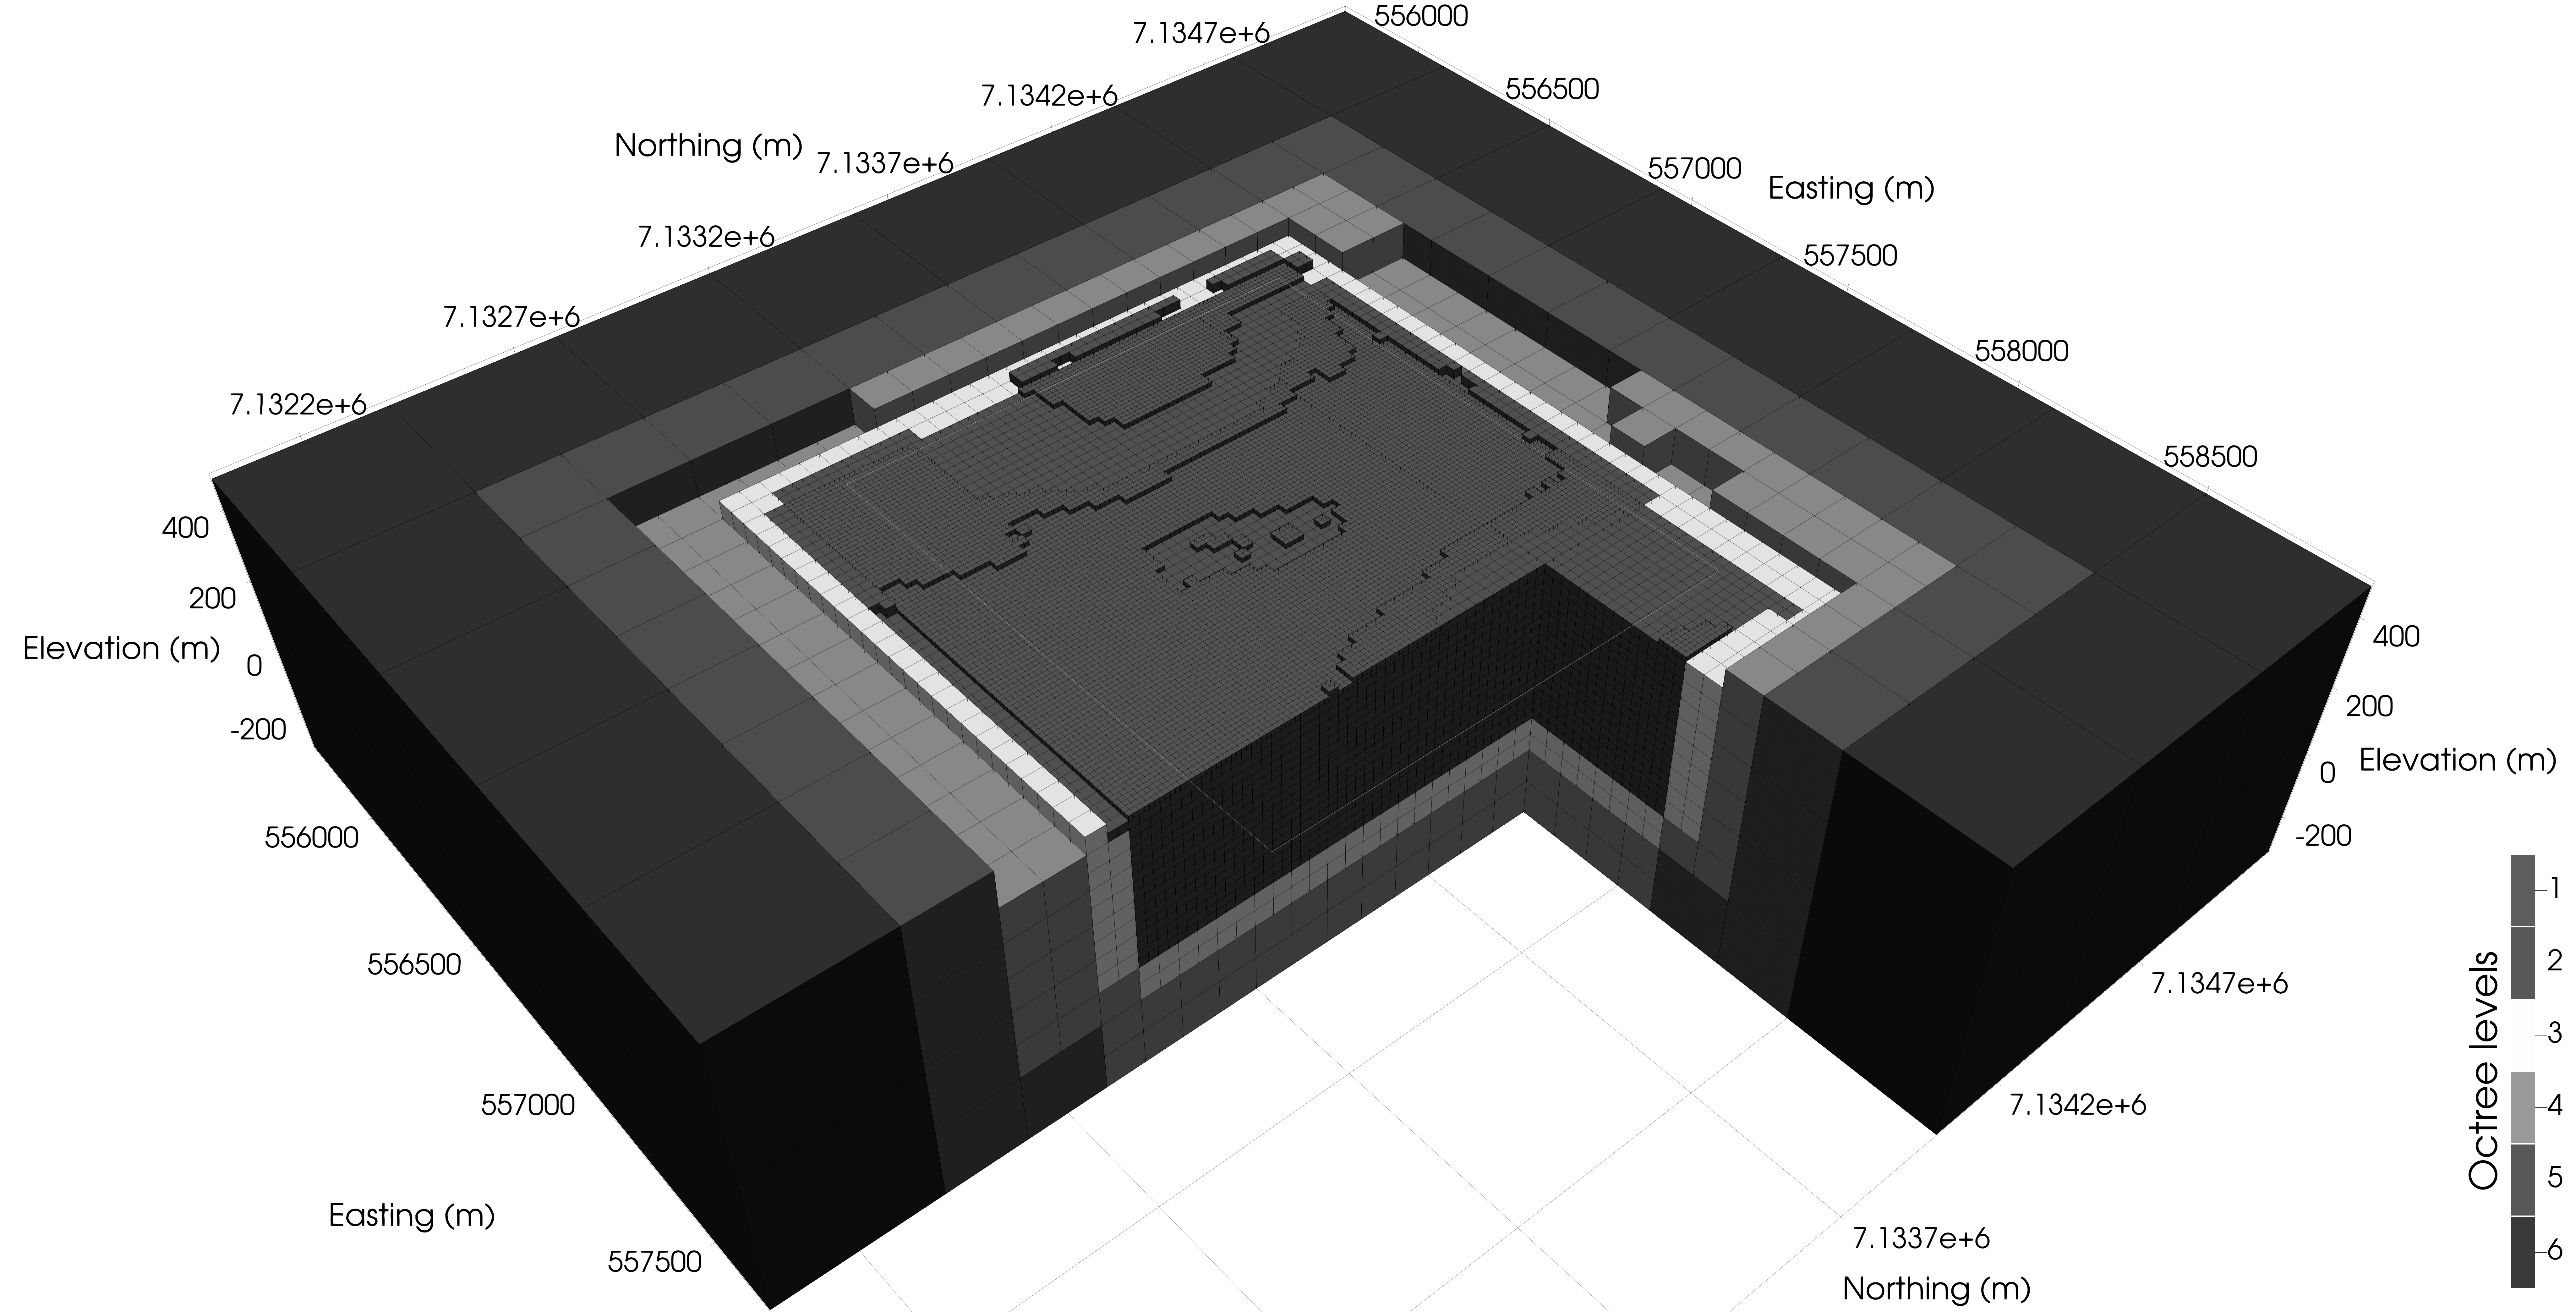
\includegraphics[width=\textwidth]{Figures/300dpi/Figure4.png}
\caption{Octree Mesh used for all the inversions. The area of interest is outlined in white. The Octree levels represent each increase in cell size (with level $1$ being the smallest cells). The volume of interest is discretized with $25$ m cubic cells (level $2$). The topography is accommodated with a layer of the smallest cells ($12.5$ m cubic cells, level $1$). The other levels ($3$ and more) serve as padding.}
\label{fig:Figure4.png}
\end{figure*}

Total field magnetic data were recorded during a VTEM survey flown in 2004 over the property, using a cesium vapor magnetometer towed $15$ m below the aircraft. The survey over the area of interest is composed of $13$ East-West flight lines $75$ m apart at an average $72$ m ground clearance.

Before the inversion, we removed a linear trend from the data using a Cauchy norm. We down-sampled the lines to one data point every $25$ m. The processed dataset is shown in Figure \ref{fig:Figure3.png}a.

A strong positive anomaly of $115$ nT is visible north of the complex. It is associated with a negative signal of $-15$ nT on the north-east; this is relatively strong for that latitude. It suggests that the data are affected by a strong remanent magnetization \citep{TKCpaper}.

To handle the different types of magnetization (induced and remanent) and the uncertainties about the remanent field direction (see \citet{TKCpaper} and the section below about modeling the petrophysical information), we use a full Magnetic Vector Inversion (MVI) with a Cartesian formulation \citep{MVI} to invert the magnetic data.

In the inversion, we assign a uniform unbiased Gaussian noise level with a standard deviation of $1$ nT; this is identical to the noise level used in \citet{TKCpaper}.

%A DIGHEM magnetic dataset has also been flown in the area but with a much lower spatial resolution above the area of interest. We decided not to include it in this study. A comparison of those two magnetic datasets can be found in \citet{TKCpaper}.

%______________________________________________________________________________
\section{Inversion Methodology}

\subsection{The geophysical inverse problem}

In our PGI approach, each iteration is similar to a smooth inversion \citep{Tutorial} that minimizes an objective function $\Phi$:

\begin{equation}
\mathop{\hbox{minimize}}\limits_{\mathbf{m}}\quad\Phi(\mathbf{m}) = \Phi_d(\mathbf{m}) + \beta \Phi_m(\mathbf{m}), \label{tikhonov}
\end{equation}
where $\mathbf{m}$ is our geophysical model, which represents physical properties on a mesh. The term $\Phi_d$ contains the sum of the various geophysical data misfits. The term $\Phi_m$ is the model regularization. The parameter $\beta$ is a positive scalar that balances the two terms.

The regularization is divided into two main terms: the smallness, which measures the distance to a reference model, and the smoothness, which regulates the variations of the model in each direction:

\begin{align}
\Phi_{m}(\mathbf{m})= \alpha_s \underbrace{\Phi_{s}(\mathbf{m})}_{\text{smallness}} + \sum_{i\in{\{x,y,z\}}}\alpha_i\underbrace{\Phi_{i}(\mathbf{m})}_{\text{smoothness}}.
\label{regularizer}
\end{align}

%\plot{Figure4.png}{width=\columnwidth}{Octree Mesh used for all the inversions. The area of interest is outlined in white. The Octree levels represent each increase in cell size (with level $1$ being the smallest cells). The volume of interest is discretized with $25$ m cubic cells (level $2$). The topography is accommodated with a layer of the smallest cells ($12.5$ m cubic cells, level $1$). The other levels ($3$ and more) serve as padding.}

\begin{figure*}
\centering
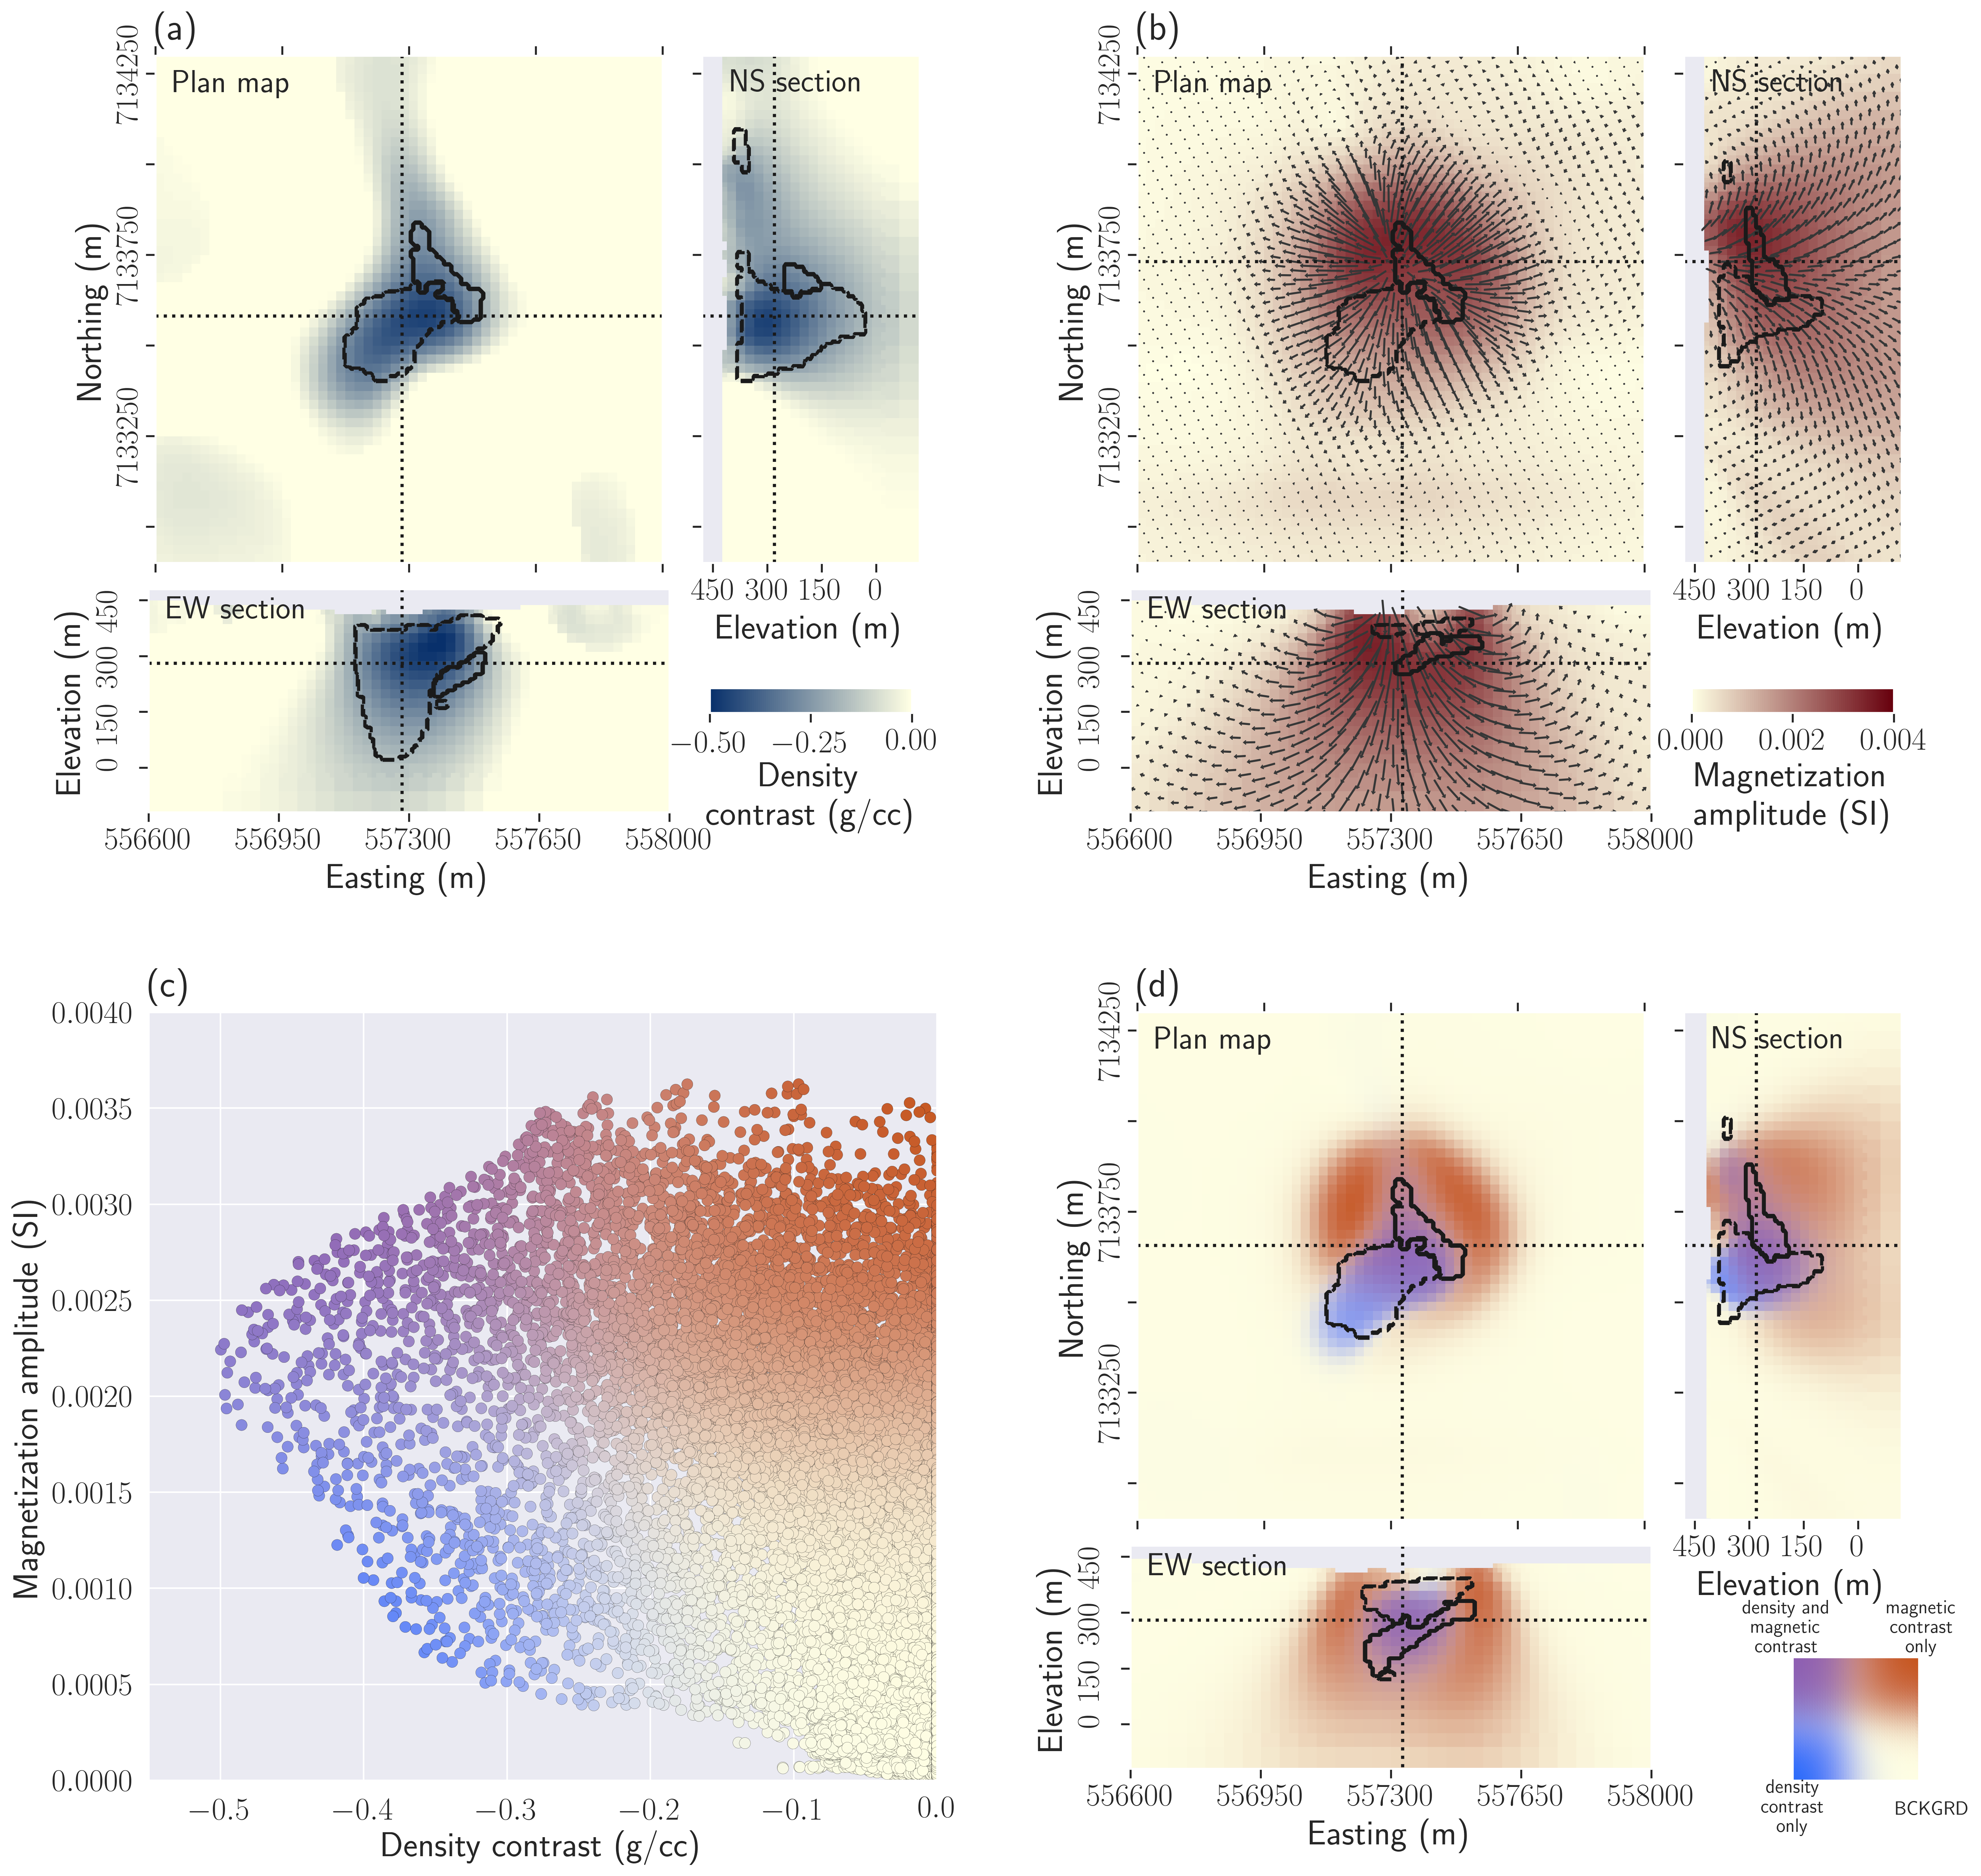
\includegraphics[width=\textwidth]{Figures/300dpi/Figure5.png}
\caption{Results of the smooth gravity inversion and MVI and post-inversion analysis. (a) Plan map, East-West and North-South cross-sections through the density model obtained by joint smooth inversion of the ground gravity and Falcon data; (b) Plan map, East-West and North-South cross-sections through the magnetic vector model obtained by MVI of the magnetic data; (c) scatter plot of the inverted density contrast and magnetization strength colored based on both physical properties; (d) colored model based on the density contrast - magnetization strength couple.}
\label{fig:Figure5.png}
\end{figure*}

All the inversions presented here are carried out with the open-source \texttt{SimPEG} package \citep{Cockett2015}. In addition, they all share the same Octree mesh (Figure \ref{fig:Figure4.png}). The use of an Octree mesh significantly speeds up the inversions while maintaining high resolution in the area of interest. All the inversions start from null half-spaces initial and reference models. For all the joint inversions, we use the computationally inexpensive strategy outline in \citet{AsticJoint} to handle multiple geophysical surveys, where the weights of the components of the total data misfit term are adjusted during the inversion until each geophysical misfit is equal or below its target value \citep{Parker}.

Smooth inversions of all the individual potential field surveys can be found in \citet{TKCpaper}. To extend that work, and to highlight the gains obtained using a PGI approach, we show two additional smooth inversion results: a smooth inversion combining the gravity and gravity gradiometry data, and a smooth MVI of the magnetic data. A post-inversion combination of the physical property models is then conducted (Figure \ref{fig:Figure5.png}).

We first perform the smooth joint inversion of the ground gravity and Falcon gravity gradiometry surveys. This is possible because both surveys are sensitive to the same physical property. Plan view and cross-sections of the recovered density model are shown in Figure \ref{fig:Figure5.png}a. The model is relatively smooth, as it is expected, and the low-density material extends well beyond the boundaries of the outline of the kimberlite units.

We then carry out the unconstrained smooth MVI to recover the magnetization vector for each cell. The MVI problem is more challenging than gravity inversions because three components need to be recovered. We use the Cartesian approach outlined in \citet{MVI} and find a smooth solution for each component. Plan view and cross-sections of the recovered model are shown in Figure \ref{fig:Figure5.png}b. Each magnetization vector is projected onto the plotting plane. The recovered vector magnetizations smoothly vary in amplitude and orientation, as it is expected. Only the large-scale region of high magnetization is predominantly visible. The cross-sections chosen for magnetization are not in the same location as those used for density because high magnetizations occur at a different location than the high-density contrast values. It is reflective of the different rock units that are generating the two responses. Close to the location of the HK unit, the vectors are oriented in a direction close to the remanent field direction estimated in \citet{TKCpaper} (inclination: $53^{\circ}$, declination: $22^{\circ}$).

To evaluate the interpretation achievable by combining our smooth inversions, we take the magnitude of the magnetization, convert it to effective susceptibility, and then plot the scatter plot of magnetization vs. density (Figure \ref{fig:Figure5.png}c). We color the points based on both the density contrast and magnetization strength (shades of blue for significant density contrast only, red for magnetic contrast and purple when both contrasts occur). The scale is provided in Figure \ref{fig:Figure5.png}d. No distinct clustering of rocks is observed. In Figure \ref{fig:Figure5.png}d, each cell in the model is assigned a color that conveys the relative values of the physical properties in that cell. For instance, a white cell denotes a background rock while a blue cell indicates a rock that has low density. Figure \ref{fig:Figure5.png}c and \ref{fig:Figure5.png}d highlight that trying to evaluate a specific volume for the PK/VK unit from these inversions would be highly dependent on the threshold value one would choose to delineate the body. Estimates obtained with clustering algorithms would have the same issues. Those limitations motivate the search for an improved solution that reproduces the petrophysical characteristics of each rock.

%\plot{Figure5.png}{width=\textwidth}{Results of the smooth gravity inversion and MVI and post-inversion analysis. (a) Plan map, East-West and North-South cross-sections through the density model obtained by joint smooth inversion of the ground gravity and Falcon data; (b) Plan map, East-West and North-South cross-sections through the magnetic vector model obtained by MVI of the magnetic data; (c) scatter plot of the inverted density contrast and magnetization strength colored based on both physical properties; (d) colored model based on the density contrast - magnetization strength couple.}

\subsection{Representing petrophysical and geological information as a Gaussian Mixture Model}

%\plot{Figure6.png}{width=\columnwidth}{Example of a Gaussian mixture model (GMM) with two properties (the axes) and two rock units (the Gaussian distributions). The main panel shows the two-dimensional GMM distribution with iso-probability level contour lines: thicker lines indicate higher probabilities. The background is colored according to the geological identification prediction. The left and bottom panels show the GMM projections in $1$D for each property, and the histogram of the fictitious samples. Figure modified from \citet{AsticJoint}.}


\begin{figure}[!ht]
\centering
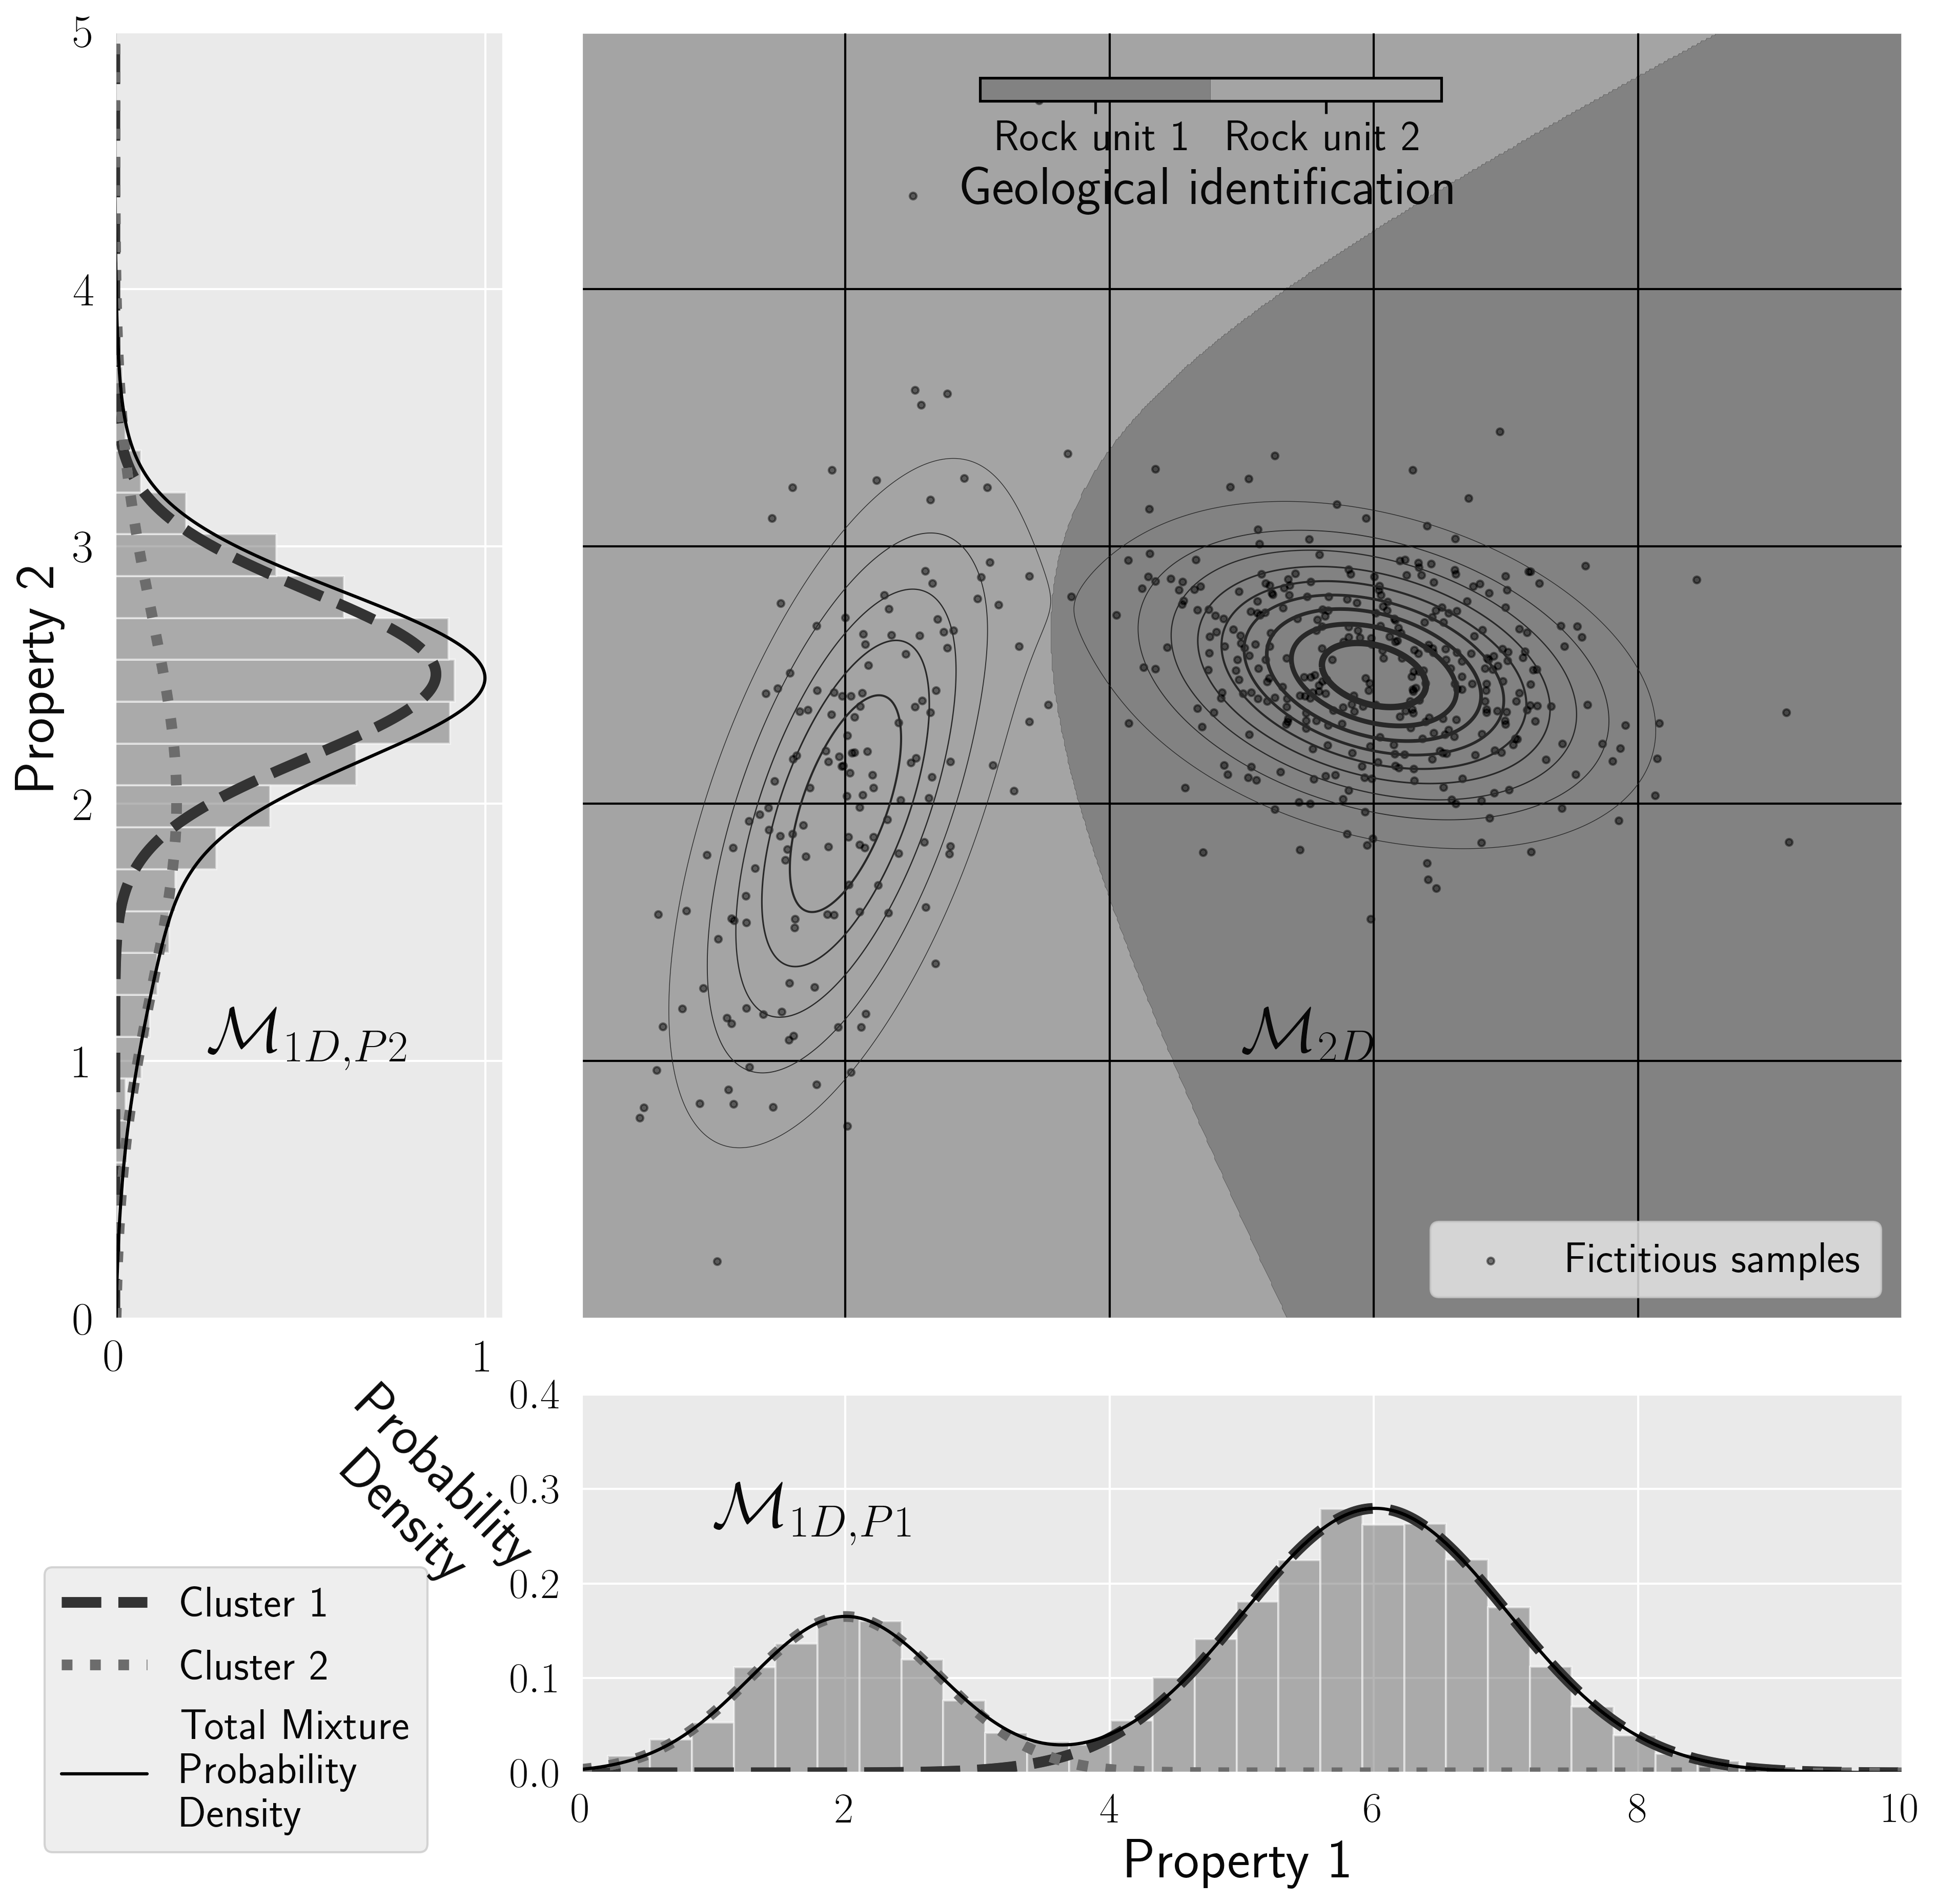
\includegraphics[width=\columnwidth]{Figure6.png}
\caption{Example of a Gaussian mixture model (GMM) with two properties (the axes) and two rock units (the Gaussian distributions). The main panel shows the two-dimensional GMM distribution with iso-probability level contour lines: thicker lines indicate higher probabilities. The background is colored according to the geological identification prediction. The left and bottom panels show the GMM projections in $1$D for each property, and the histogram of the fictitious samples. Figure modified from \citet{AsticJoint}.}
\label{fig:Figure6.png}
\end{figure}

To include physical property information into the inversion, we model the petrophysical signature of each rock unit by a Gaussian probability distribution. Each unit (indexed $j$, for a total of $c$ units) is defined by the mean of its physical properties ($\mathbf{\mu}_j$) and a covariance matrix linking the various physical properties ($\Sigma_j$). Computations of those values based on samples are shown in equations \ref{MLE-means} to \ref{MLE-cov}. Measured physical properties for a sample $s$ belonging to rock unit $j$ is represented by $\mathbf{x}_{s \in j}$. The number of available samples for rock unit $j$ is denoted $s_j$.

%Let's consider a given petrophysical dataset with $n$ samples, denoted $\{\mathbf{x}_i,i=1..n\}$. Each $\mathbf{x}_i$ represents the various measured physical properties for the sample $i$. For each sample we know its current geological classification. This is denoted by $j=1..c$ where $c$ the number of distinct geological units. A sample $i$ belonging to unit $j$ is noted $\mathbf{x}_{i\in j}$. With known labels, the Gaussian distribution parameters for each unit $j=\{1..c\}$ are given in equations \ref{MLE-weights} to \ref{MLE-cov} (respectively its mean $\ma
%tbf{\mu}_j$, its covariance matrix $\Sigma_j$, plus its relative proportion $\pi_j$).


\begin{align}
\mathbf{\mu}_j &= \frac{1}{s_j}\sum_{s=1}^{s_j}\mathbf{x}_{s \in j}.
\label{MLE-means}
\end{align}

\begin{align}
\Sigma_j & = \frac{1}{s_j}\sum_{s=1}^{s_j}(\mathbf{x}_{s \in j}-\mathbf{\mu}_j)(\mathbf{x}_{s \in j}-\mathbf{\mu}_j)^T.
\label{MLE-cov}
\end{align}

The Gaussian distribution representing each unit $j$ is denoted $\mathcal{N}(\cdot | \mathbf{\mu}_j, \Sigma_j)$. We regroup the petrophysical and geological information of all the known units in the form of a Gaussian mixture model (GMM) (equation \ref{GMM}), which is a sum of the Gaussian signatures weighted by the prior probability of encountering the rock unit $j$ at the location $i$ (denoted $\pi_{i,j}$). This last parameter does not have to be precise and has minimal effects when set constant everywhere. Allowing those probabilities to vary depending of the location provides an additional way to include geological information \citep{Giraud2017} and we use this functionality later in this paper. Thus the probability function to observe a physical properties data point $\mathbf{x}$ at location $i$ can be written:

\begin{align}
&\mathcal{P}(\mathbf{x}_i) = \sum_{j=1}^c \pi_{i,j} \mathcal{N}(\mathbf{x}_i|\mathbf{\mu}_j,\Sigma_j). \label{GMM}
\end{align}

A fictitious example of a GMM with two physical properties (the axes) and two rock units (the Gaussian distributions) is shown in Figure \ref{fig:Figure6.png}. Each Gaussian represents the petrophysical signature of a rock unit for the two physical properties. The background color highlights the most likely rock unit for any given values of the physical properties; we refer to this classification as the geological identification.
% (denoted $z$). %which we denote $\mathbf{z}$.

%The geological identification is denoted $\mathbf{z}$. Given an unlabeled data point $\mathbf{x}_0$, its geological identification $z_0$ takes the value of the geological unit with the highest probability (see equation \ref{MAP_z_physProp}).

%\begin{align}
%&z_0 = \mathop{\hbox{argmax}}\limits_{z \in \left\{1..j\right\}}\mathcal{P}(\mathbf{x}_0|z)\mathcal{P}(z) \label{MAP_z_physProp}\\
%&\text{with:} \nonumber \\
%&\mathcal{P}(z) = \pi_z \text{ and}\label{weight_z_prior} \\
%&\mathcal{P}(\mathbf{x}_0|z)=\mathcal{N}(\mathbf{x}_0| \mathbf{\mu}_{z},\Sigma_{z}).
%\end{align}

\subsection{Key concepts for Petrophysically and Geologically guided Inversions (PGI)}

As put forward in \citet{ggz389}, we can build upon the objective function in equation \ref{tikhonov} to incorporate petrophysical and geological information (represented as a GMM) to better constrain our physical property models. This prior knowledge is contained within the smallness term (equation \ref{regularizer}). The PGI problem is nonlinear and the objective function is minimized iteratively \citep{Tutorial}. At each iteration, the reference model $\mathbf{m}_{\text{ref}}$ and the smallness weights $W_{s}$ are updated based on our knowledge of the petrophysical and geological characteristics. Our augmented smallness term then takes the following form:

\begin{align}
&\Phi_{small}(\mathbf{m}) = \frac{1}{2}\sum_{i=1}^n||W_{s}(z_i)(\mathbf{m}_i-\mathbf{m}_{ref}(z_i))||_2^2, \label{smallness_petro}\\
\end{align}
with:
\begin{align}
&z_i = \mathop{\hbox{argmax}}\limits_{j} \pi_{i,j}~\mathcal{N}(\mathbf{m}_i|\mathbf{\mu}_j, \Sigma_j), \label{membership} \\
\end{align}
\begin{align}
&\mathbf{m}_{\text{ref}}(z_i) = \mathbf{\mu}_{z_i}, \label{mref_update}\\
\end{align}
\begin{align}
&W_{s}(z_i) = \Sigma_{z_i}^{-1/2}\text{diag}(\mathbf{w}_{{i}}), \label{Ws_update}
\end{align}
where $z_i$ denotes the geological identification, and $\mathbf{w_i}$ are sensitivity weights for each physical property at cell $i$, for a total number of $n$ cells.
The update can be understood as a classification of each cell of the mesh into its most likely geological unit based on the current geophysical model and prior knowledge (equation \ref{membership}). This classification defines our quasi-geologic model, and it is used to create a new reference model and smallness weights with the following procedure. For the reference model $\mathbf{m}_{\text{ref}}$, each cell is assigned the petrophysical mean values of the identified rock unit (equation \ref{mref_update}). The smallness weights $W_{s}$ at each cell include the covariance matrix of the physical properties for the identified rock unit to represent the expected variations and correlations (equation \ref{Ws_update}); they also include the sensitivity weights for each physical property, necessary for potential fields inversions \citep{Li1996, Li1998, Li2001}. This iterative update of the smallness term guides the inversion towards reproducing the petrophysical signature of each rock unit while fitting the geophysical data.

%______________________________________________________________________________
\section{Modeling the petrophysical information at DO-$27$}

Qualitative information about the physical properties of the various rock types found at DO-$27$ was used during previous studies relying on Tikhonov inversions \citep{TKCpaper,TKCEM,TKCIP}. For our work, we need more quantitative information from field samples. We obtained $20$ samples of the various kimberlite facies from Peregrine Diamonds Ltd. $11$ samples of PK, $4$ of VK, and $5$ of HK were sent to the Geological Survey of Canada Paleomagnetism and Petrophysics Laboratory, Victoria, BC, for characterizing the physical properties of each unit. In the following material, we discuss those measurements and how we compiled information into a form that allows us to generate a GMM. Means and standard deviations summarizing the petrophysical characteristics of each rock unit are provided in Table \ref{tbl:gmmtable}.

\subsection{Density information}
\label{pkvkdensitysection}

\begin{figure*}%*
\centering
\includegraphics[width=\textwidth]{Figures/300dpi/Figure7.png}
\caption{Design of the PK/VK unit density signature in the GMM. (a) Cross-section of the density contrast estimate for the PK/VK unit from \citet{TechnicalReport}; (b) Scatter plot, density contrast versus elevation of the cells, of the cross-section shown in panel (a). We fit a Gaussian on each unit (PK/VK and background); the contour lines represent iso-probability levels from the resulting GMM, and the background color indicates the geological identification.}
\label{fig:Figure7.png}
\end{figure*}%*

The HK samples were mechanically competent, and 5 densities were obtained: $2.764$, $2.867$, $2.435$, $2.632$ and $2.677 \text{ g/cm}^3$. Those samples yield an average density of $2.675 \text{ g/cm}^3$, which is similar to the estimated background density of $2.67 \text{ g/cm}^3$ \citep{TKCpaper}. The HK unit is deemed indistinguishable from the background from the density standpoint. Their mean density contrast is thus set to $0 \text{ g/cm}^3$. The density of the background unit is, however, assigned a smaller standard deviation.

The PK and VK units are highly porous and mechanically weak. Unfortunately, this prevented density information from being obtained from several samples. Those that were successfully analyzed are believed to be associated with more competent and denser samples. Those samples are thus deemed unrepresentative of the kimberlite unit in general and were not used. Instead, we rely on density measurements taken by Peregrine Diamonds Ltd during the drilling programs. A block model of the density of PK was built based on those measurements \citep{TechnicalReport}. To include this information in our inversion, we digitized the published cross-section through this block model (Figure \ref{fig:Figure7.png}a). Assuming a background density of $2.67 \text{ g/cm}^3$, the density contrast is $\sim-1.1 \text{ g/cm}^3$ at $400$ m elevation and changes linearly to achieve a value of $\sim-0.5 \text{ g/cm}^3$ at $200$ m elevation.
This cross-section provides enough information for us to characterize the density signature of the PK/VK unit and build a GMM. To include the linear trend of density contrast with depth, we include the elevation as a fixed parameter in our coupling term. We generate a two-dimensional GMM (density contrast and elevation) that is consistent with the observations (shown in Figure \ref{fig:Figure7.png}b along with the scatter plot of the cross-section). The elongated and tilted shape of the Gaussian distribution representing the PK/VK unit accounts for the correlation of density contrast with depth. On the contrary, the background (and HK) density values are assumed to be independent of the depth. This is modeled by assigning a high standard deviation for the elevation of those units; their assigned mean elevation is then of no consequence in the inversion. The long vertically elongated shape of the Gaussian distribution for the background unit manifests the independence of the density contrast with respect to the elevation for that unit. Means and standard-deviations characterizing the density contrast of each rock unit are provided in Table \ref{tbl:gmmtable}.

%\plot{Figure7.png}{width=\textwidth}{Design of the PK/VK unit density signature in the GMM. (a) Cross-section of the density contrast estimate for the PK/VK unit from \citet{TechnicalReport}; (b) Scatter plot, density contrast versus elevation of the cells, of the cross-section shown in panel (a). We fit a Gaussian on each unit (PK/VK and background); the contour lines represent iso-probability levels from the resulting GMM, and the background color indicates the geological identification.}

\subsection{Magnetic susceptibility information}

%plot{Figure8.png}{width=\columnwidth}{(a) Magnetic measurements in the laboratory; (b) $2$D projections of the $3$D GMM of the Cartesian components of the magnetic vector estimated for the background and HK units; contour lines represent iso-probability levels of the GMM, and the background color indicates the geological identification. The background unit is limited to the space defined by the small ellipsoid.}


\begin{figure*}%*
\centering
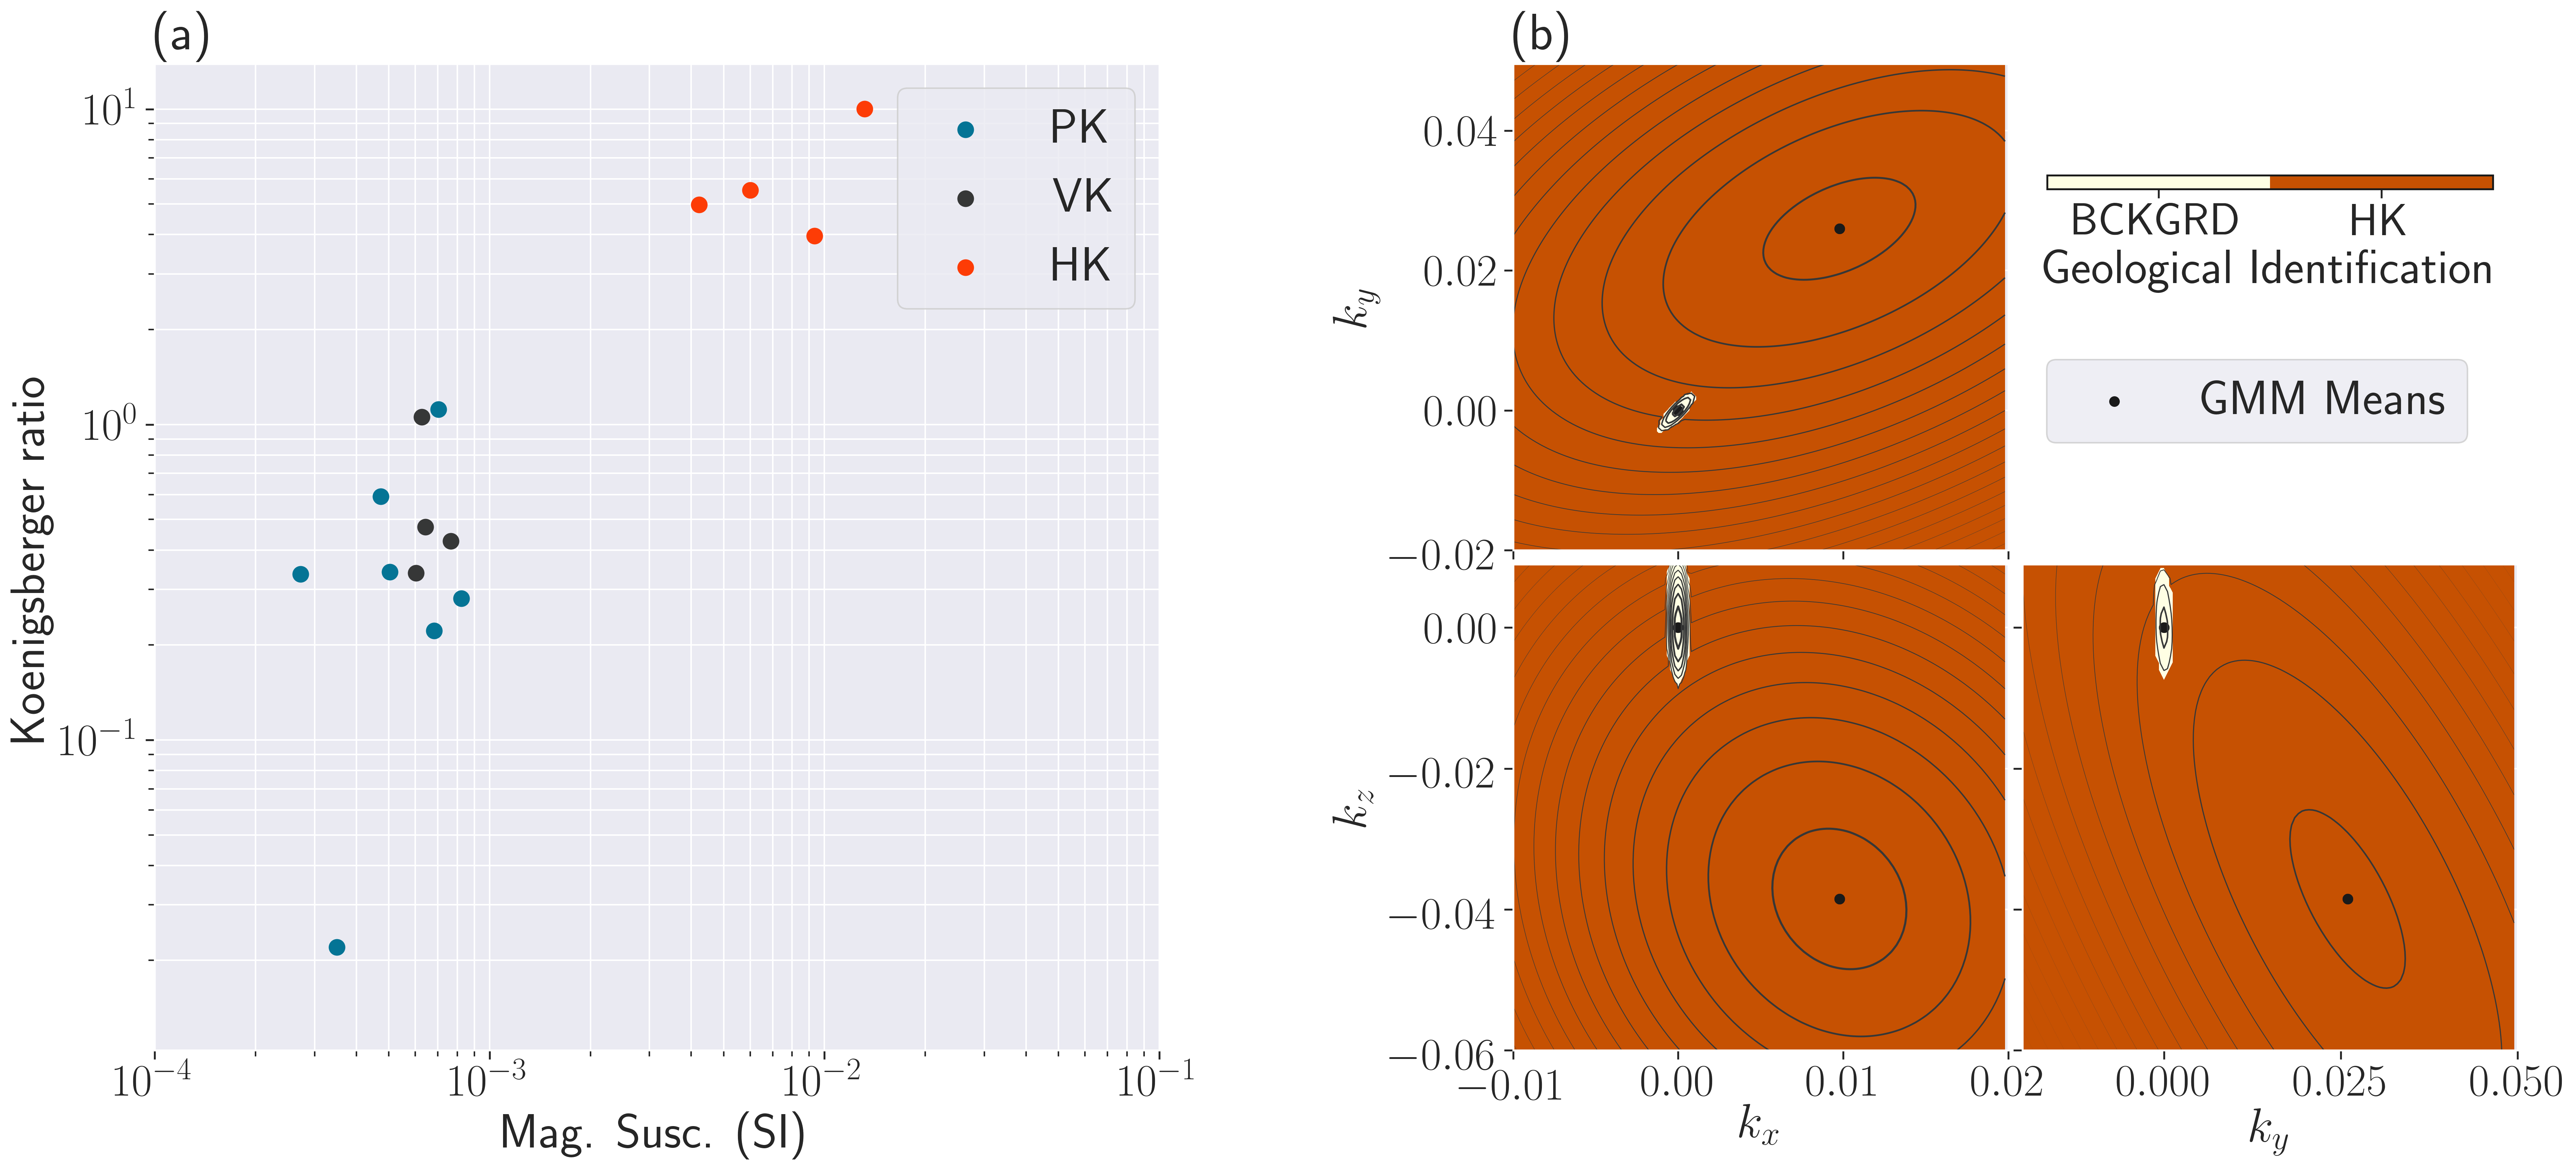
\includegraphics[width=\textwidth]{Figures/300dpi/Figure8.png}
\caption{(a) Magnetic measurements in the laboratory; (b) $2$D projections of the $3$D GMM of the Cartesian components of the magnetic vector estimated for the background and HK units; contour lines represent iso-probability levels of the GMM, and the background color indicates the geological identification. The background unit is limited to the space defined by the small ellipsoid.}
\label{fig:Figure8.png}
\end{figure*}%*

For our samples, both the induced magnetization and the strength of the remanent field were measured (Figure \ref{fig:Figure8.png}a). The strength of the remanent field was given in the form of a Koenigsberger ratio \citep{Koenigsberger}. The magnetic susceptibility of the samples spans a wide range of values, which is consistent with the fact that magnetic susceptibility generally has a logarithmic distribution \citep{LogMag,LogMag2,Enkin}.

If we are given the remanent magnetization direction, we can estimate an effective susceptibility $k_\text{eff}$ for the magnetic vector of each unit:

\begin{equation}
k_\text{eff} = k||\hat{u}_{earth}+Q \frac{{B}_{lab}}{{B}_{earth}}\hat{u}_{rem}||_2,
\end{equation}
where $k$ is the measured magnetic susceptibility (purely inductive magnetic response), $\hat{u}_{earth}$ is the unit vector of the Earth's magnetic field direction at DO-$27$, $Q$ is the Koenigsberger ratio, $B_{earth}$ is the IGRF magnetic field at DO-$27$, ${B}_{lab}$ is the amplitude of the magnetic field used in the laboratory for the measurements ($59000$ nT) and $\hat{u}_{rem}$ is the unit vector of the remanent magnetization direction.

The PK and VK units have a small magnetic susceptibility and are weakly remanent. The effective susceptibility of those two units, assuming that the remanent field is aligned with the current Earth's magnetic field, is estimated at $8 \cdot 10^{-4}$ SI.

Only $4$ samples of HK were measured for their magnetic response. Their Koenigsberger ratios are close to $10$. Hence the magnetic response of the HK unit in the data is essentially due to remanent magnetism. However, we need an estimation of the remanent magnetization orientation of the HK unit to obtain an effective susceptibility. \citet{TKCpaper} obtained an estimation of a $53^{\circ}$ inclination and $22^{\circ}$ declination by cross-correlation of the vertical and total gradients of the reduced to pole data. The uncertainty of that estimation is about $10^{\circ}$ for each angle. Using these estimated angles, we obtain an average effective susceptibility of $5 \cdot 10^{-2}$ SI for the HK unit.

%The mean and standard deviation values of the log-effective magnetic susceptibility, inclination, and declination for each rock unit are provided in

%Given the measured magnetic susceptibilities, and after modeling the magnetic response of each body based on the geologic model, we estimated that the magnetic response of PK/VK was likely negligible compared to the response of HK. The magnetic signal observed at DO-$27$ is thus assumed to be dominated by HK, and mainly from its remanent magnetization. Under these assumptions, the estimation of a $53^{\circ}$ inclination and $22^{\circ}$ declination obtained by \citet{TKCpaper} by cross-correlation of the vertical and total gradients of RTP data seems a good approximation for the remanence direction of HK.

The mean and standard deviation values of the log-effective magnetic susceptibility, inclination, and declination for each rock unit are provided in Table \ref{tbl:gmmtable}. Those values define Gaussian distributions of the magnetization parameters in a spherical coordinates system with a logarithmic distribution for magnetization amplitudes. Ideally, we would like to invert for a log-susceptibility model, but that poses challenges since the very low susceptibilities do not generate a substantial signal in the magnetic field data. We, therefore, revert to the usual practice of inverting for magnetic susceptibility on a linear scale. Our MVI algorithm inverts for each Cartesian component of magnetization $\left\{k_x,k_y,k_z\right\}$. For PGI, we need to represent the magnetization in a GMM. We thus need to obtain means and covariance matrices for $\left\{k_x,k_y,k_z\right\}$. To this end, we appeal to random numerical sampling methods. For each rock unit, we randomly sample, from their Gaussian distribution in spherical coordinates, log-effective susceptibility, and angles triplets. We convert those synthetic samples to Cartesian values and use them to estimate the desired means and covariances (equations \ref{MLE-means} and \ref{MLE-cov}).

%As we provide petrophysical information to the inversion, we choose to use the simpler linear Cartesian formulation, which is
%We did use a spherical formulation during our experiments. But, as we give a gaussian distribution to respect, keeping the linear, cartesian problem appeared simpler for equivalent outcomes.

%For each unit, we have obtained thus far log-amplitude and angles mean and standard deviation values. Those values define Gaussian distributions of the magnetization parameters in a spherical coordinate system using the estimated angles and effective susceptibilities and their respective uncertainties, estimated from the samples for the magnetic susceptibility and the RTP data analysis for the angles. We convert those synthetic samples to Cartesian values and then estimate the desired means and covariances (equations \ref{MLE-means} and \ref{MLE-cov}). We sample the amplitudes in log-susceptibility since that is the space in which Gaussian distributions best represent magnetic susceptibility. We also assume that the amplitude and the angles are independent of each other (null values for the non-diagonal covariance matrix coefficients).

The resultant GMM for magnetic parameters can be visualized in Figure \ref{fig:Figure8.png}b. The resulting probability distributions appear elongated and tilted, indicating correlations between the Cartesian components of magnetization. Given the measured magnetization and uncertainties, the weakly magnetic PK and VK units are difficult to distinguish from a non-susceptible background due to the nearby highly magnetic HK unit. The PK/VK unit and the background have thus been grouped under "background" in Figure \ref{fig:Figure8.png}b.
%Moreover, the weakly magnetic PK and VK units are spatially close to the highly magnetic HK unit, making them potentially difficult to be distinguished from a non-susceptible background.
%and after modeling the magnetic response of each body based on the geologic model, we estimated that the magnetic response of PK/VK was likely negligible compared to the response of HK. T


\subsection{Petrophysical characterization summary}

\begin{table}
\centering
\label{tbl:gmmtable}
\caption{Physical properties and elevation parameters for each rock unit. For the PK/VK-pipe unit, the values are reported without the rotation of the Gaussian distribution caused by the linear trend with depth. Notation and units: $\bar{x}$: mean of $x$; $\sigma_x$ standard-deviation of $x$; $\rho$: density contrast ($\text{g/cm}^3$); $z$: elevation (meter); $k$: effective magnetic susceptibility ($\log10$ SI); $\theta$: inclination ($^{\circ}$); $\phi$: declination($^{\circ}$).}
% \scalebox{0.75}{
%\rotatebox{90}{
% {\renewcommand{\arraystretch}{1.} %<- modify value to suit your needs
\begin{tabular}{|c|c|c|c|c|c|c|c|c|c|}
\hline
Rock unit & $\bar{\rho}$ & $\sigma_\rho$ & $\bar{z}$ & $\sigma_z$ & $\bar{k}$ & $\sigma_k$ & $\bar{\theta}$ & $\bar{\phi}$ & $\sigma_{\theta, \phi}$\\
\hline
Background & 0 & 0.03 & 290 & 180 & -6 & 0.24 & 83.8 & 19.5 & 10 \\
\hline
PK/VK & -0.75 & 0.07 & 290 & 75 &-3.1 & 0.24 & 83.8 & 19.5 & 10\\
\hline
HK & 0 & 0.1 & 290 & 180 & -1.3 & 0.33 & 53 & 22 & 10 \\
\hline
PK-minor & -0.3 & 0.1 & 360 & 10 & -3.1 & 0.24 & 83.8 & 19.5 & 10\\
\hline
\end{tabular}
%}
%}
%}
\end{table}

We have defined, in terms of density and magnetization, the characteristics of the background and main kimberlite units identified in the DO-$27$ pipe. Table \ref{tbl:gmmtable} summarizes the quantitative values used to define the GMMs for the various inversions we conduct. Information about a new unit, PK-minor, is also reported. This unit is used in our final inversion, and more details are given in the multi-physics PGI section.

Regarding density, the background and HK units are both assigned a $ 0 \text{ g/cm}^3$ mean density contrast, while the PK/VK unit presents a mean density that varies with depth. The background and HK units are indistinguishable, and the gravity anomaly is primarily due to the PK/VK unit. Thus, carrying out an inversion just for a density contrast model with PGI only requires a petrophysical GMM consisting of two rock units (background and PK/VK).

%The HK and background units are indistinguishable in an inversion only for density contrast. The source of the gravity anomaly only consists of

A similar situation occurs for magnetic properties. The HK unit is dominant, and its magnetization is nearly two orders of magnitude larger than the PK/VK unit. Any inversion that focuses purely on magnetic data would have challenges delineating the PK/VK unit from the background in the presence of the HK unit. Thus carrying out a PGI solely for a magnetic vector model only necessitates a petrophysical GMM with two rock units (background and HK).

%From the perspective of their magnetic properties, the background and the PK/VK units are deemed indistinguishable, while the HK unit is highly magnetic and remanent.

%This lack of distinction in terms of a single physical property leads us to run the single-physics inversions with only two rock units: the background and one kimberlite unit (PK/VK for the gravity inversion and HK for the magnetic inversion, see next section).

Although only two rock units are justified when inverting for a single type of physical property, the situation changes when we consider the density and magnetic characteristics together. As illustrated in Figure \ref{fig:Figure6.png}, units that appear indistinguishable in one physical property ($1$D space, property $2$) can be distinct when considering a higher-dimensional petrophysical space (the $2$D space). In our case, the background, PK/VK, and HK units are distinct in the $5$D space composed of density, elevation, and the three magnetic vector components. The multi-physics inversions take advantage of that higher dimensionality of the GMM to recover all three units at once (see the multi-physics PGI section). We now carry out the single-physics and multi-physics PGI to illustrate these ideas.

%For our final inversion, we also introduce a new unit PK-minor to represent shallow occurrences of kimberlites whose density signature appears to differ from the main PK/VK unit found in the pipe. Its characteristics were chosen after running a range of inversions, and more details are given in the multi-physics PGI section.


%______________________________________________________________________________
\section{Single-physics PGIs}

We now invert, with the PGI approach, datasets that are connected by a single physics. We recover a density model from gravity and gravity gradiometry data using the information that the density of the PK/VK unit increases with depth. From the magnetic data, we recover a magnetic vector model that is compatible with our knowledge about the magnetization of the HK unit. The density and magnetization models are then combined to highlight the limitation of single-physics and post-inversion classification approaches in delineating the two kimberlite units.

%We display in this section, the results obtained by performing single physics inversion, gravity, and magnetic, respectively, with the addition of petrophysical information.

\subsection{Joint PGIs of the ground gravity and Falcon airborne gravity gradiometry data}

%\plot{Figure9.png}{width=\textwidth}{Inversion result with PGI of the ground gravity and Falcon surveys using the density signature of PK/VK; (a) Plan map, East-West and North-South cross-sections through the recovered density contrast model along each plane. The dotted line represents the location of each cross-section; (b) Comparison between the petrophysical GMM (contours plot) used to regularize the inversion and the recovered density contrast model (scatter plot).}


\begin{figure*}%*
\centering
\includegraphics[width=\textwidth]{Figures/300dpi/Figure9.png}
\caption{Inversion result with PGI of the ground gravity and Falcon surveys using the density signature of PK/VK; (a) Plan map, East-West and North-South cross-sections through the recovered density contrast model along each plane. The dotted line represents the location of each cross-section; (b) Comparison between the petrophysical GMM (contours plot) used to regularize the inversion and the recovered density contrast model (scatter plot).}
\label{fig:Figure9.png}
\end{figure*}%*

We first jointly invert the ground gravity and airborne gravity gradiometry with the addition of our petrophysical model to include our knowledge about the expected density contrasts and their variations with depth. The obtained density model is shown in Figure \ref{fig:Figure9.png}a, and can be compared with the result obtained by jointly inverting the two datasets but without a petrophysical constraint (Figure \ref{fig:Figure5.png}). The trend with depth can be seen in the scatter plot in Figure \ref{fig:Figure9.png}b. Each survey has reached its target misfit.

A single body, reproducing the PK/VK petrophysical signature, is sufficient to fit the gravity data. The horizontal outline of this PK/VK body is in reasonable agreement with the geologic model, except for a region north of the pipe. The bottom of the PK/VK body is also relatively well constrained. On the North-South cross-section, we can distinguish low-density material in the upper surface (around $-0.1 \text{ g/cm}^3$, above $300$ m elevation) that lies above the northern extension of the identified PK/VK volume. That anomaly may be related to other minor kimberlite occurrences and is still identified as background in the quasi-geologic model (Figure \ref{fig:Figure9.png}b).

%a weak density anomaly on top of the PK/VK tip;

%______________________________________________________________________________
\subsection{Magnetic Vector Inversion of the airborne magnetic data with PGI}

%\plot{Figure10.png}{width=\textwidth}{Result of the petrophysically guided MVI. (a) Plan map, East-West, and North-South cross-sections through the magnetic vector model along each plane. The dotted line represents the location of each cross-section. The dark arrows represent the magnetization direction and strength; (b) Comparison between the petrophysical GMM (contour plots) used to constrain the magnetic vector model and the recovered magnetic vector model (scatter plots). The background unit appears in the plots as the small ellipsoid. Background cells are all within that small portion of the parameter-space. The geological identification is used to color the background of the plot.}


\begin{figure*}%*
\centering
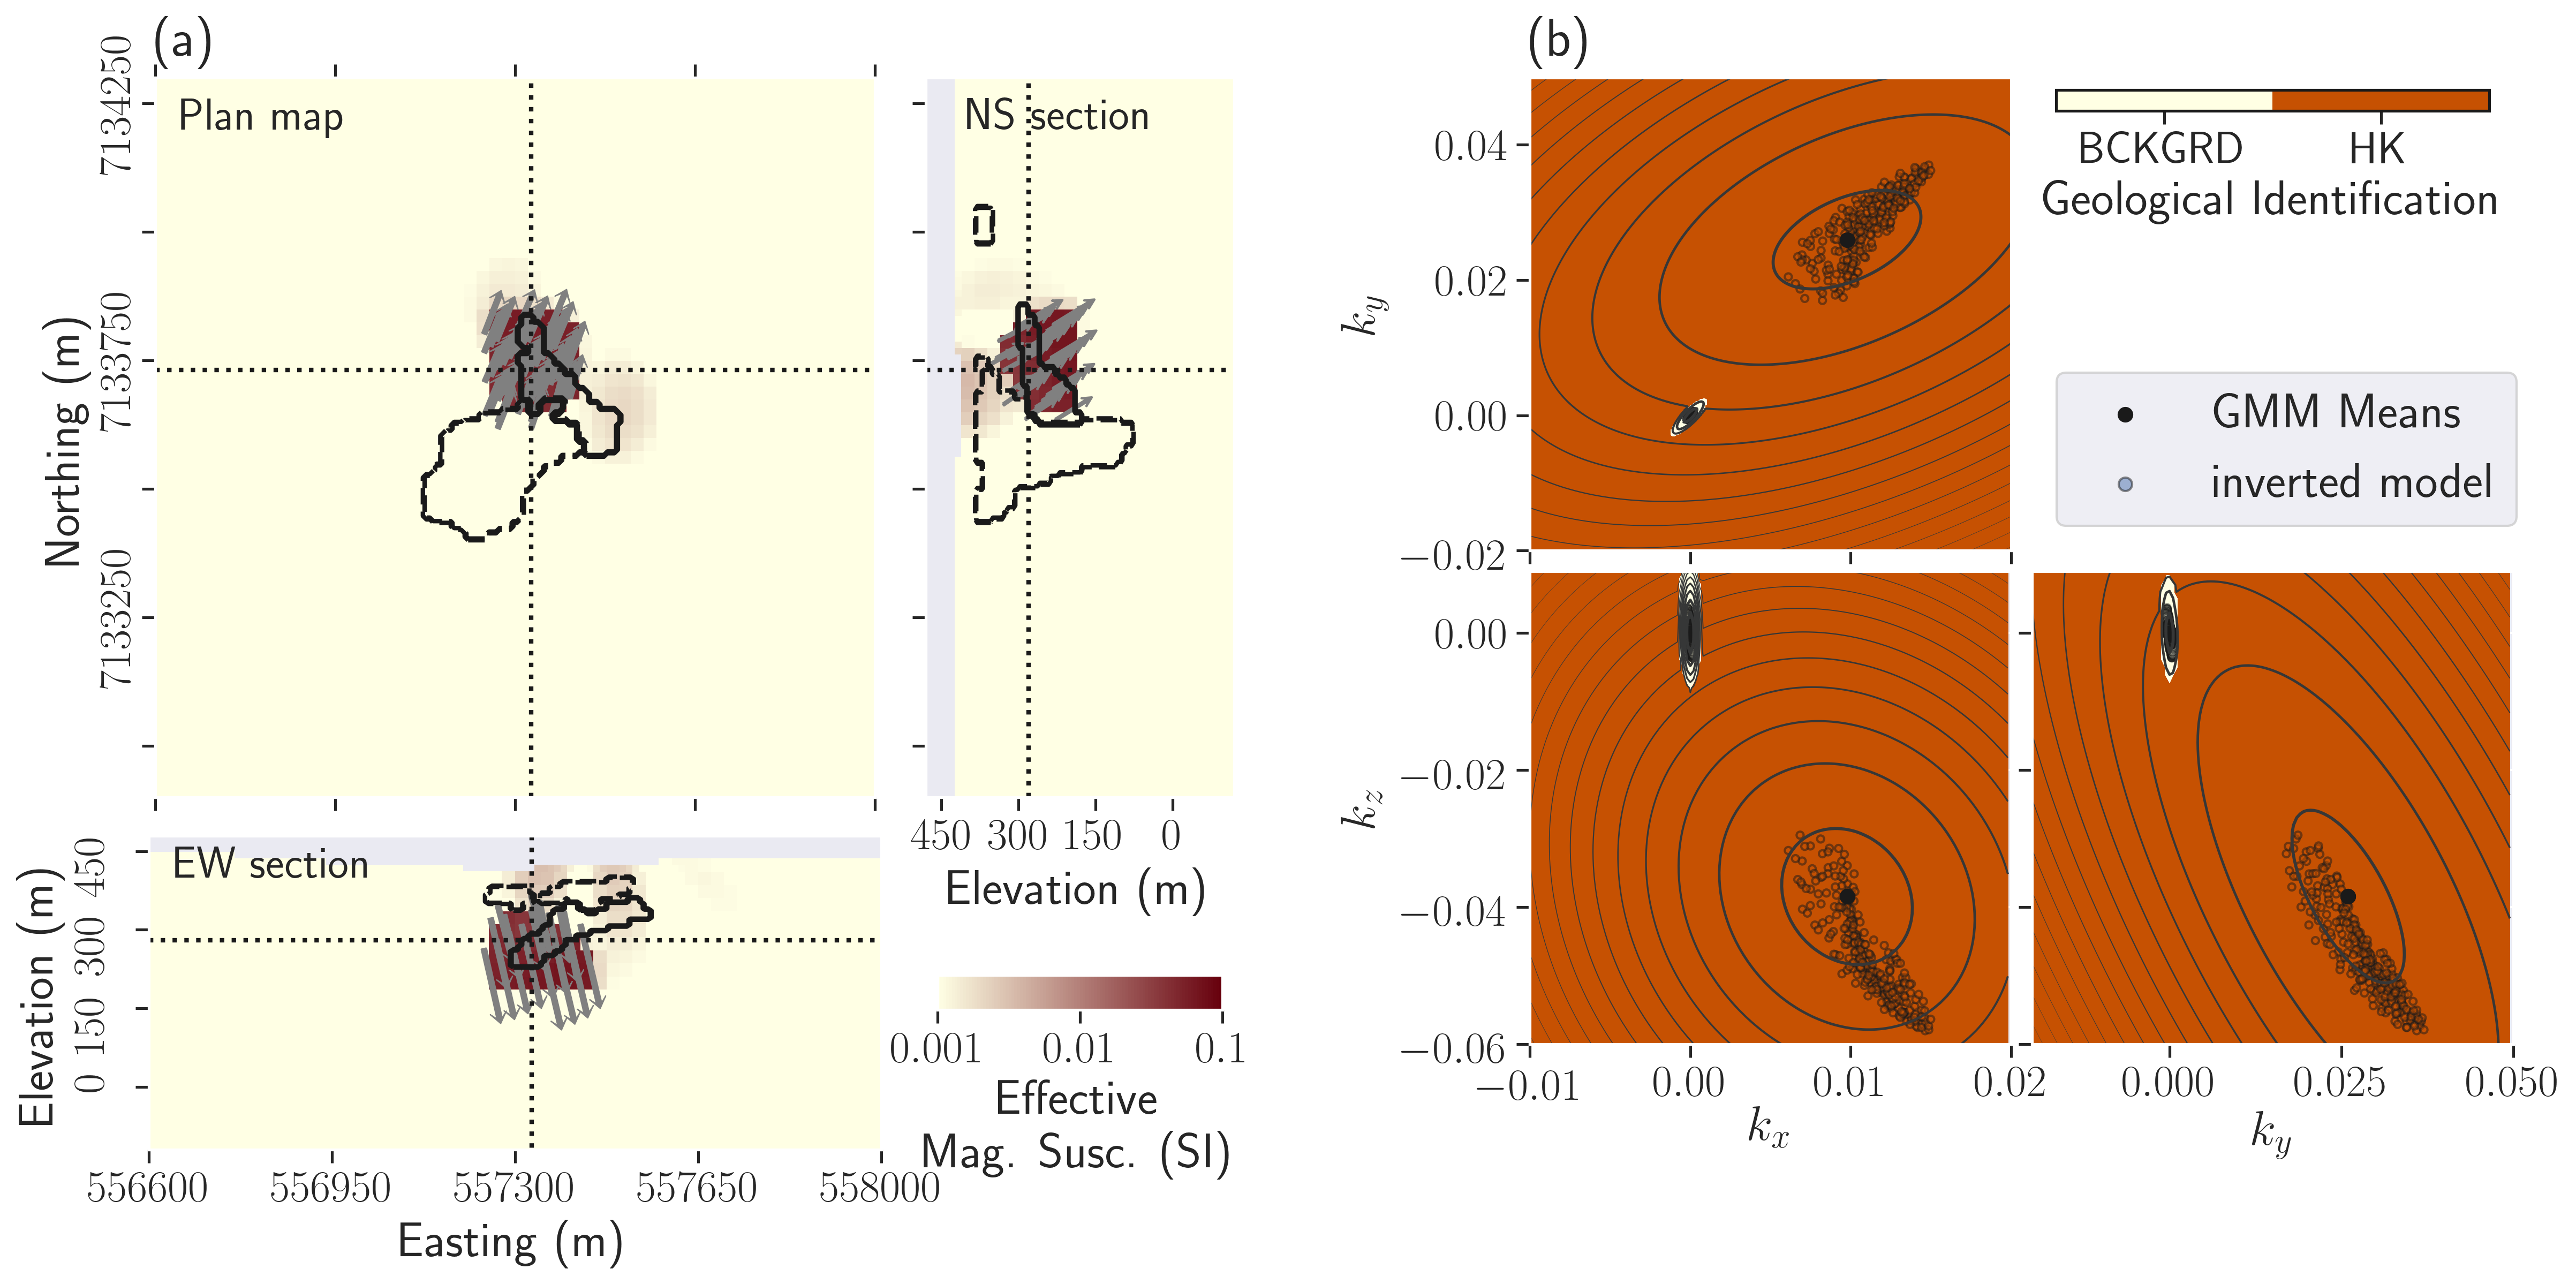
\includegraphics[width=\textwidth]{Figures/300dpi/Figure10.png}
\caption{Result of the petrophysically guided MVI. (a) Plan map, East-West, and North-South cross-sections through the magnetic vector model along each plane. The dotted line represents the location of each cross-section. The dark arrows represent the magnetization direction and strength; (b) Comparison between the petrophysical GMM (contour plots) used to constrain the magnetic vector model and the recovered magnetic vector model (scatter plots). The background unit appears in the plots as the small ellipsoid. Background cells are all within that small portion of the parameter-space. The geological identification is used to color the background of the plot.}
\label{fig:Figure10.png}
\end{figure*}%*

Here we invert the magnetic data using a MVI approach to recover each component $\left\{k_x,k_y,k_z\right\}$ of a magnetic vector. The inclusion of petrophysical information, through the GMM, ensures we are reproducing the signature of the HK unit.

The result of the inversion with petrophysical knowledge is shown in Figure \ref{fig:Figure10.png}a. We recover a well-defined, compact magnetic body with consistent magnetic orientation reproducing the modeled petrophysical signature of HK (Figure \ref{fig:Figure10.png}b). The location of the HK unit coincides well with that obtained from drillholes, except that the eastern side of the mapped HK unit is not recovered, and no dip is visible. No anomaly related to PK/VK is visible in the magnetic vector model.
%, and it is indistinguishable from the background with the current approach.

%______________________________________________________________________________
\subsection{Post-inversion classification of the individually obtained density and magnetic vector models}

%\plot{Figure11.png}{width=\columnwidth}{Combination of the individual petrophysically guided inversions. The "UNDEFINED" area corresponds to a volume where both high density and magnetic contrasts were found, corresponding to no known rock units signature.}


\begin{figure}
\centering
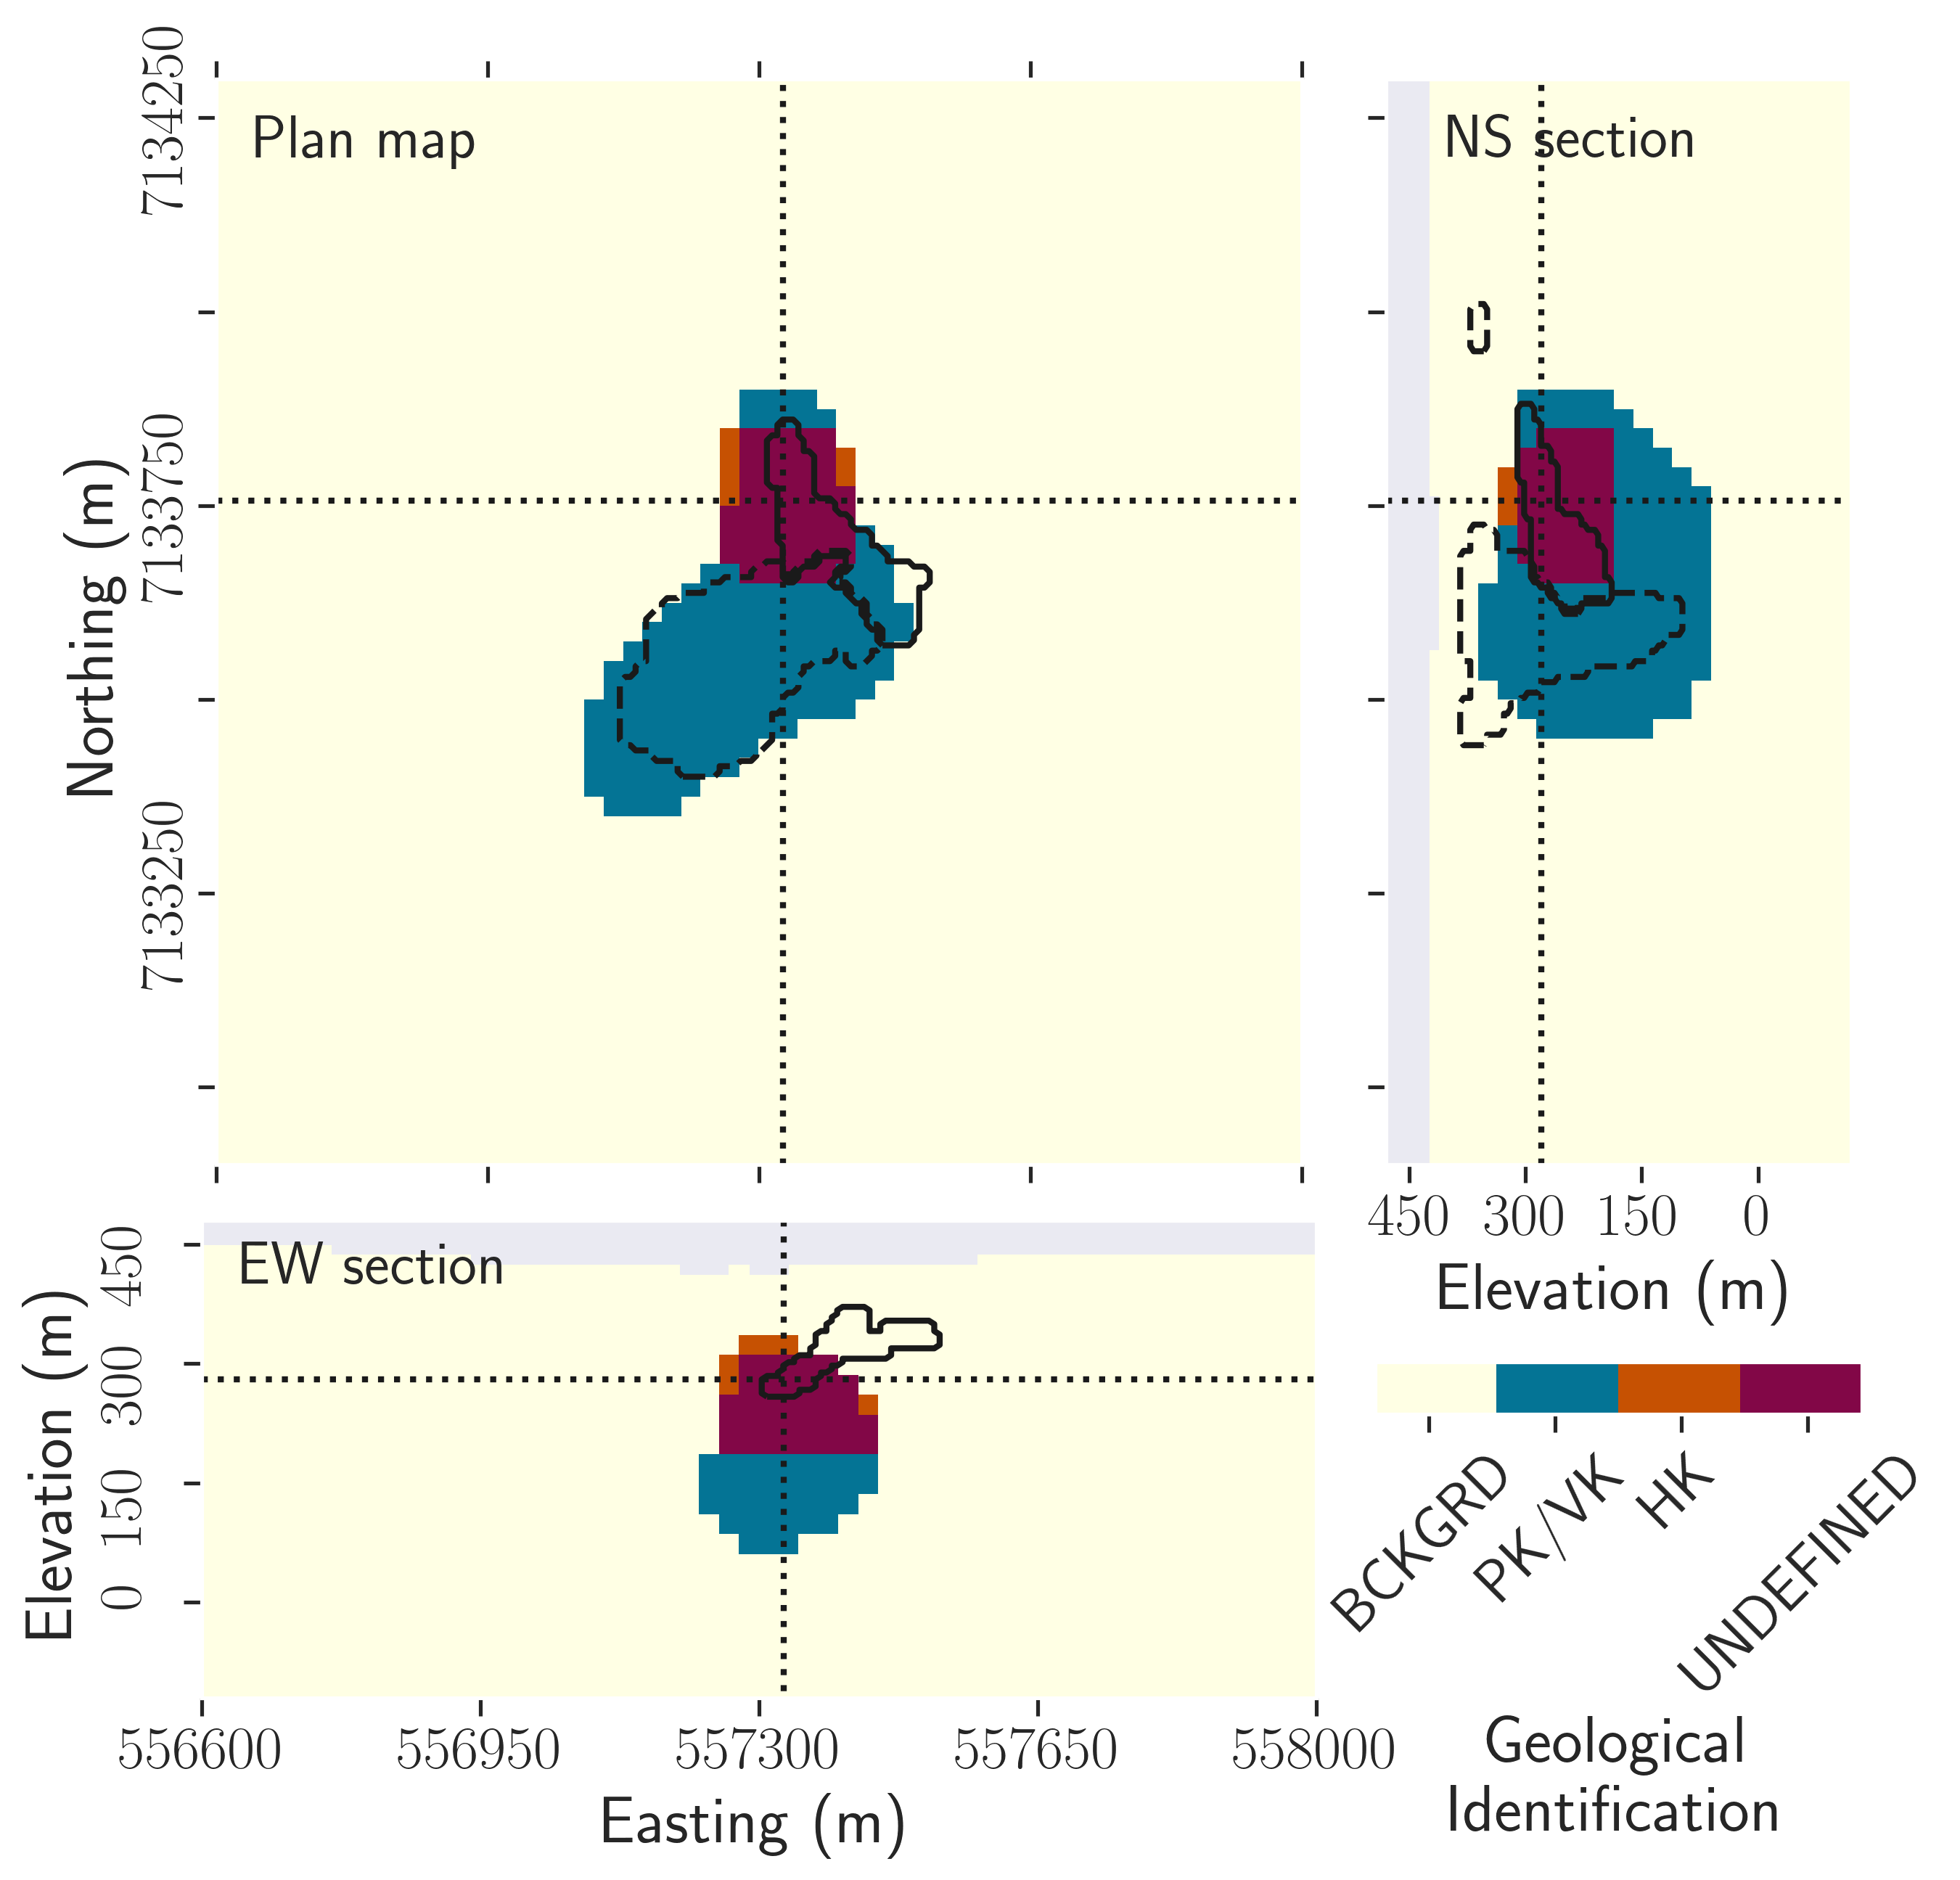
\includegraphics[width=\columnwidth]{/Figures/300dpi/Figure11.png}
\caption{Combination of the individual petrophysically guided inversions. The "UNDEFINED" area corresponds to a volume where both high density and magnetic contrasts were found, corresponding to no known rock units signature.}
\label{fig:Figure11.png}
\end{figure}

At this stage, we have obtained two physical property models.
One is a density model that reproduces both gravity datasets and the PK/VK density signature. The HK unit is not necessary to explain the gravity data and is considered to be indistinguishable from the background regarding its density.
The second is a magnetic vector model that globally reproduces the magnetic data and HK magnetic signature. In this inversion, the PK/VK unit is deemed to be indistinguishable from the background regarding its magnetic susceptibility.

Combining the two models (Figure \ref{fig:Figure11.png}) highlights the limits of post-inversion classification with single-physics inversions of geophysical datasets. Even with the addition of petrophysical information and the dominance of each unit in each inversion, the combination of the two models shows an important overlap between the recovered PK/VK and HK units (marked as the "UNDEFINED" area). This volume, actually covering most of the recovered HK unit, is found to have both strong density and magnetic contrasts. This signature disagrees with our petrophysical knowledge of the area.

To overcome this, we propose to invert all three surveys (ground gravity, airborne gravity gradiometry, and airborne magnetic) together with all five coupling parameters (density contrast, elevation, and the three components of the magnetic vector).


%______________________________________________________________________________
\section{Multi-physics PGIs}

In this section, we use our PGI approach to invert all three datasets along with the petrophysical information about the rock units. We first consider three rock units (background, PK/VK, and HK) to form the GMM. We then further refine the quasi-geologic model by adding a fourth unit and geological \textit{a priori} information, based on drillholes, into a subsequent inversion to recover desired geological features.

%we present the result of the multi-physics inversions, coupled with petrophysical information by the GMM. The first inversion shows the result obtained by merging the approach taken into the previous single-physics inversions. Based on that result, we further refine the quasi-geologic model by adding ad hoc geological a priori information, based on drillholes, into a subsequent inversion to recover desired geological features.

\subsection{Multi-physics inversion with petrophysical information}

%\plot{Figure12.png}{width=\textwidth}{Results of the multi-physics PGI with three rock units. (a) Plan map, East-West, and North-South cross-sections through the density contrast model; (b) Magnetic vector model. The gray arrows are the projections of the magnetization directions (unit vector) on the plane for the kimberlite units; (c) Presentation of the $5$-dimensional GMM: visualization of all possible $2$D projections. Comparison with the recovered model represented as the scatter plots of the four physical properties of the geophysical model and the elevation; (d) Resulting quasi-geologic model from the multi-physics PGI with three rock units.}


\begin{figure*}%*
\centering
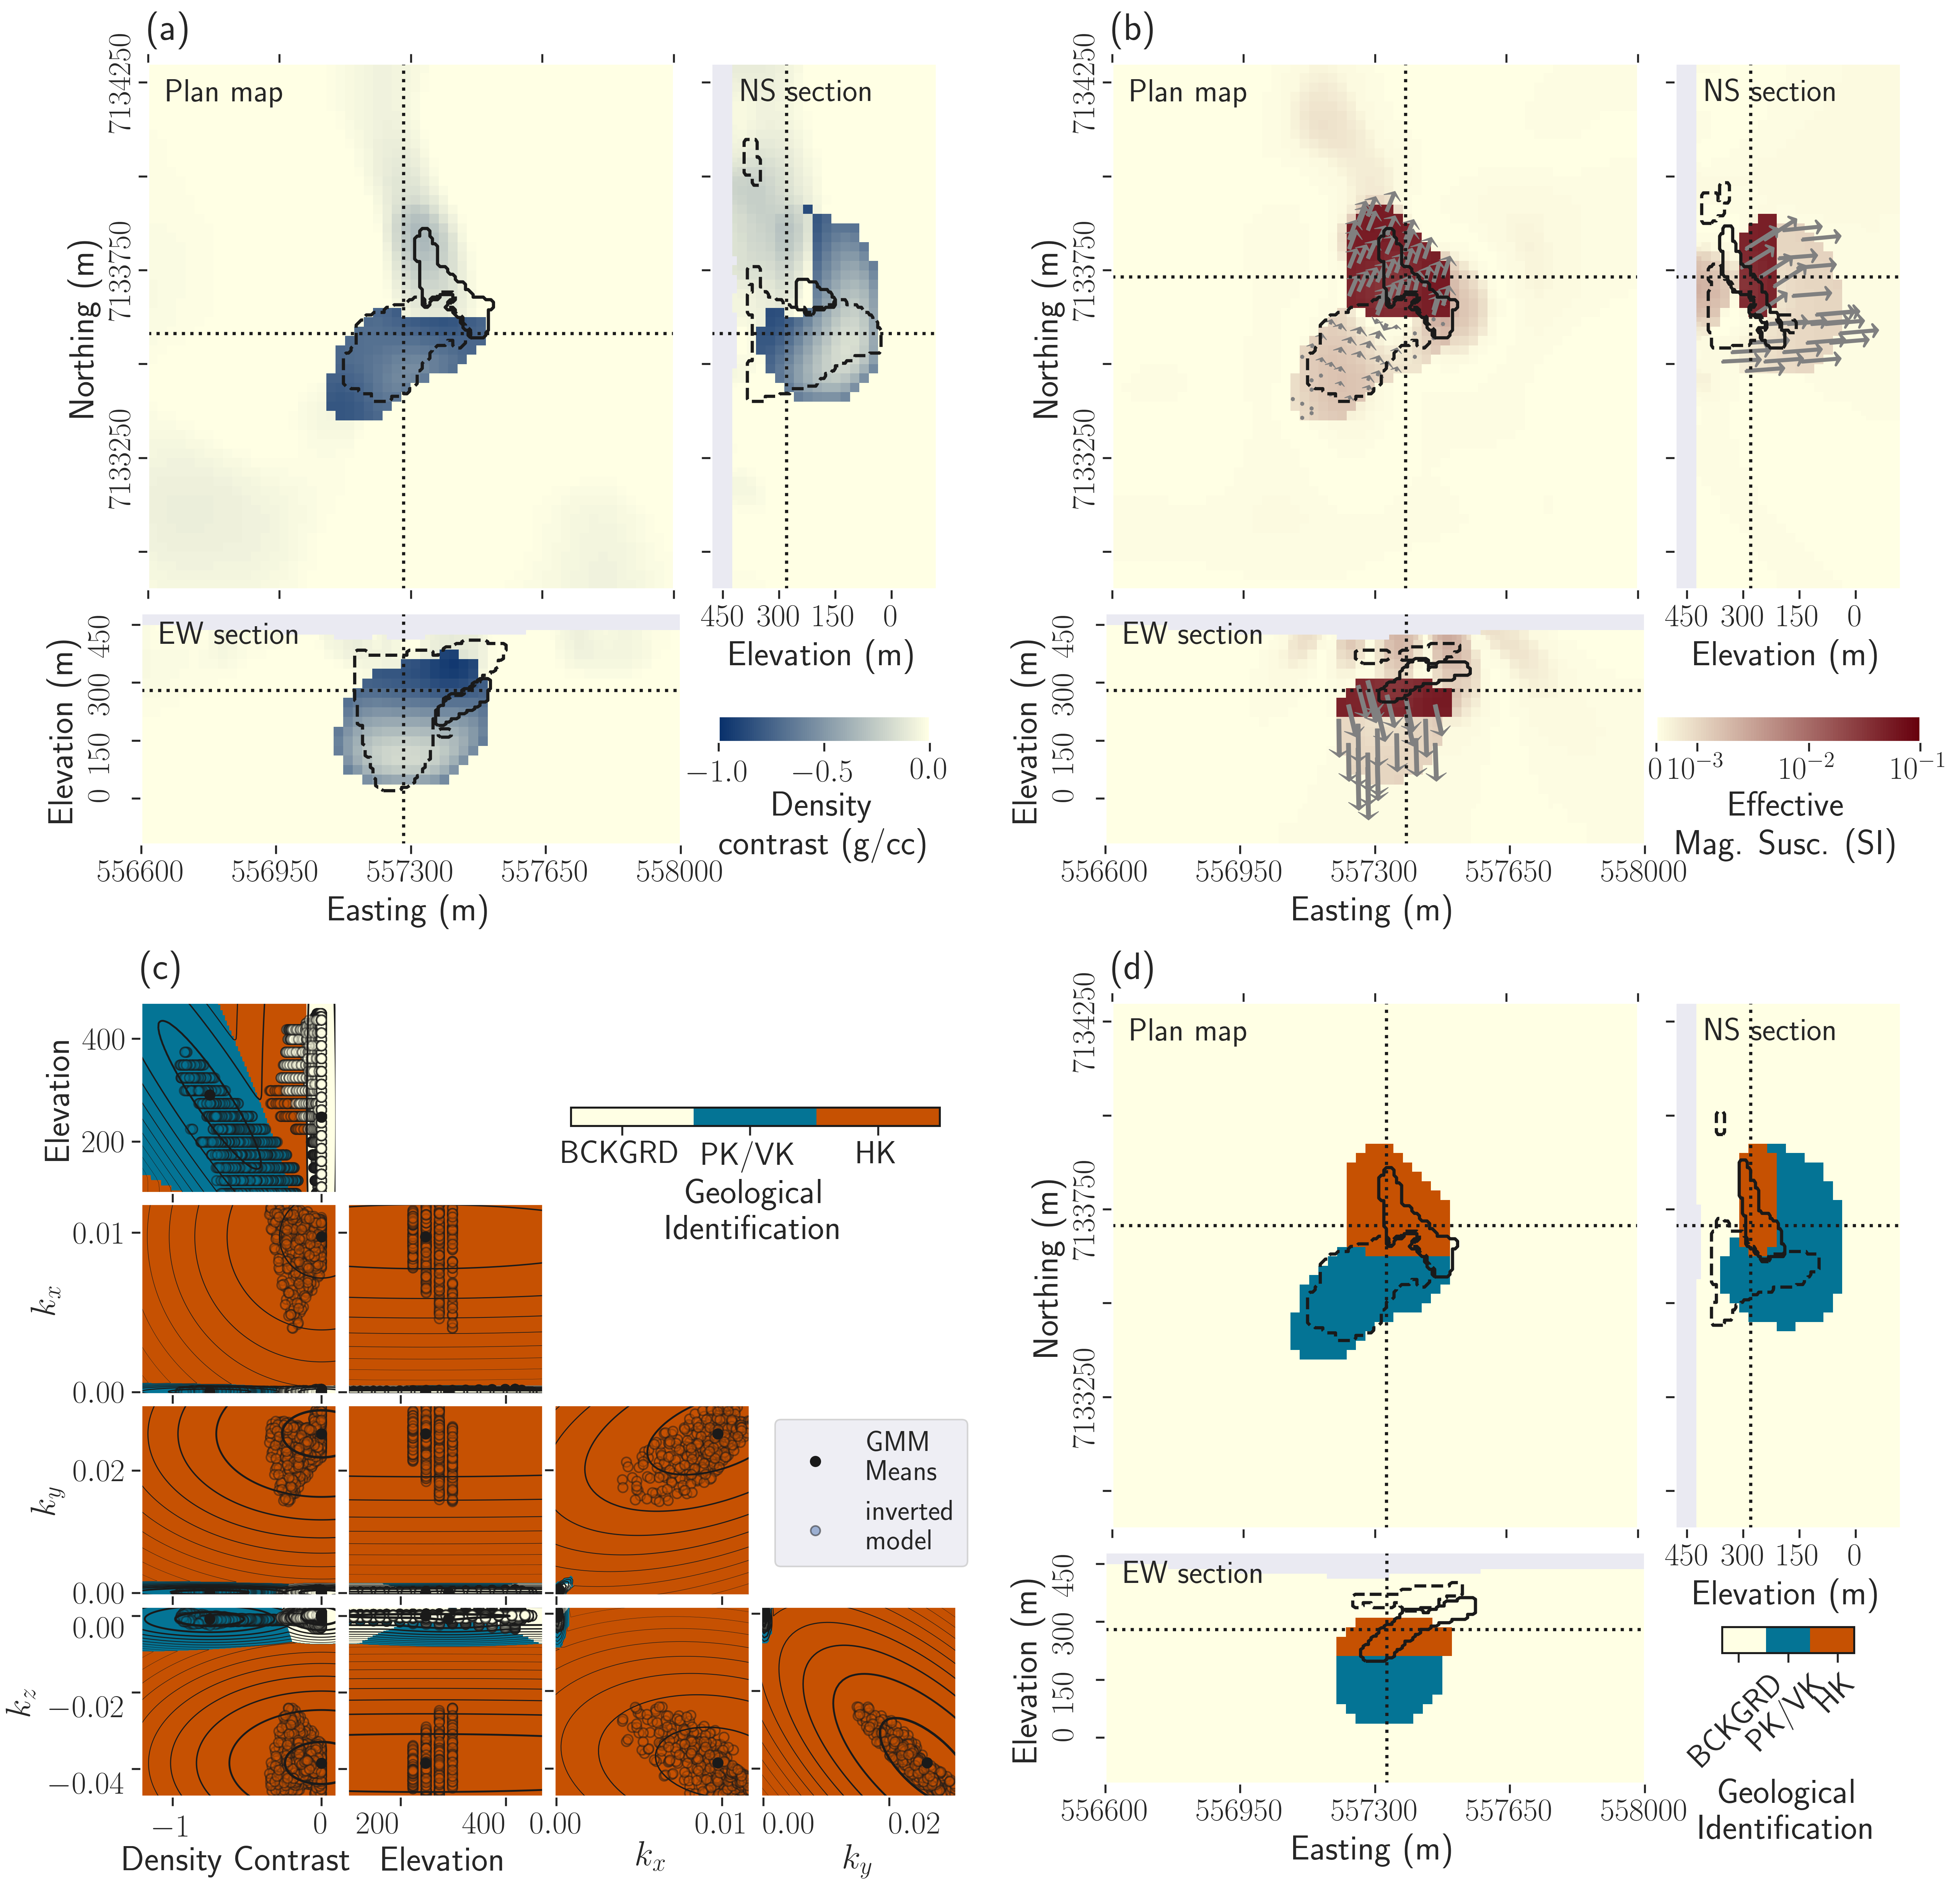
\includegraphics[width=\textwidth]{Figures/300dpi/Figure12.png}
\caption{Results of the multi-physics PGI with three rock units. (a) Plan map, East-West, and North-South cross-sections through the density contrast model; (b) Magnetic vector model. The gray arrows are the projections of the magnetization directions (unit vector) on the plane for the kimberlite units; (c) Presentation of the $5$-dimensional GMM: visualization of all possible $2$D projections. Comparison with the recovered model represented as the scatter plots of the four physical properties of the geophysical model and the elevation; (d) Resulting quasi-geologic model from the multi-physics PGI with three rock units.}
\label{fig:Figure12.png}
\end{figure*}%*

The multi-physics PGI result is presented in Figure \ref{fig:Figure12.png}. The improvement over the single-physics inversions, both smooth and petrophysically guided, is quite pronounced. The overlapping of the units observed by combining single-physics inversions has been resolved by the multi-physics inversion, which reproduces the full five-dimensional petrophysical distribution.

Figure \ref{fig:Figure12.png}c presents the $5$D GMM by showing all possible $2$D projections. The values of the physical properties model are well clustered around the prescribed means and along determined trends. The dimensionality increase of the GMM allows us to define three distinct units (background, PK/VK, and HK), with their specific signature for all physical properties. The multi-physics inversion recovers an HK unit with a mean density contrast of about $-0.12~\text{g/cm}^3$. Similarly, the magnetic signature of the recovered PK/VK unit is now distinguishable from the background; it has a mean effective susceptibility of $1.06 \cdot 10^{-3}$ SI, which is close to the expected value of $8 \cdot 10^{-4}$ SI. The PK/VK magnetization is also oriented along the Earth's magnetic field, as required. This orientation differs from the remanent magnetization given to the HK unit. This difference in orientation can be seen in Figure \ref{fig:Figure12.png}b. It is only with the multi-physics inversion approach that we can define two clear kimberlite facies (Figure \ref{fig:Figure12.png}d).

\subsubsection{Comparison with a geologic model from drilling}

Now that we have obtained a quasi-geologic model containing all three major units that reproduce the geophysical datasets and petrophysical information, we can compare it to the geologic model built from drillholes (Figure \ref{fig:Figure12.png}d).

%The surface outlines of the PK/VK unit from the geophysical and geological data are in good general agreement. The addition of petrophysical information well constrains the bottom extension and the surface outline. The most important differences occur in the northern region. Same as in the individual gravity inversion, the gravity data require a northern extension of the PK/VK kimberlite units. However, this northern extension of the PK/VK unit has been pushed down at depth in the joint inversion with magnetic data. It happens due to the recovery of the HK unit close to the surface, in agreement with the geologic model. The density contrast of the HK unit is assumed to be null, thus requiring low-density material at depth. As a result, the PK/VK unit lies beneath the HK in our joint inversion. This observation seems to disagree with drill results that reported granitic rocks beneath HK. We still recover low-density material north of the pipe at the near-surface. However, it is not identified as belonging to the PK/VK unit. That weak density anomaly is likely related to minor occurrences of PK facies that have been intercepted north of DO-$27$ (such as illustrated by pocket-like structures in the geologic model outline).

%The near-surface part of the HK unit is well recovered. The unit seems to continue further West than in the geologic model. Few drillholes have been logged in that area, which can explain that missing feature in the geologic model. On the other hand, the inversion underestimates the mapped East portion of HK, where the highest residual misfits are observed. No dip is distinguishable from the inversion model, which image the HK unit as a horizontal blocky body.

The HK unit is reasonably well localized, but not all details are reproduced by the inversion. In reality, the HK unit is a thin, dipping body that we image as a horizontal body. We miss a portion of the unit that is mapped on the East, and our unit continues further West than that in the geologic model. We note, however, that few drillholes have been logged in the western area, so there might be some uncertainty in the geologic model.

The PK/VK unit, which is diamondiferous, is in good agreement with the geologic model over the region of the pipe. Importantly, the bottom extension of that unit seems to have been well-constrained by incorporating the petrophysical data. The major discrepancy between our model and the geologic model is in the northern region, where PK/VK material has been placed beneath the HK unit. This result contradicts drill results that show no PK/VK occurrence beneath the HK unit. To understand how this happened, we need to re-examine the gravity inversion results and the information that is input into the PGI.
In the inversion of the gravity data alone, low-density material is required in the region north of the pipe. However, in the magnetic inversion, that region is occupied by the HK unit, which is assumed to have no density contrast with the background. In the multi-physics inversion, any low-density material required to fit the gravity data must, therefore, be put either at depth or in a near-surface layer. However, because of the assumed dependence of density and elevation, the density of a near-surface layer must be very low. The inability to fit the gravity data with that very low-density shallow layer provides no alternative for the inversion except to put anomalous density material at depth. To resolve this inconsistency with geology, we introduce another geologic unit and carry out a new multi-physics inversion that includes expanded a priori information.


\subsection{Adding geological information into the multi-physics inversion}

The previously obtained model from a multi-physics inversion with petrophysical information allows us to recover distinct units with the required petrophysical signature. However, several features of the quasi-geologic model are in disagreement with the geological knowledge from drillholes, namely the northern extension of the PK/VK pipe below the HK unit and the lack of dip for the HK unit.

To overcome those issues, we revise our assumptions of what to add as a priori information into the inversion. We have assumed so far that near-surface occurrences of PK facies had similar density characteristics as the PK/VK unit found in the DO-$27$ pipe. Those near-surface occurrences, which showed up in the inversion results as smooth density contrast features, were still categorized as background (Figures \ref{fig:Figure9.png} and \ref{fig:Figure12.png}). It is an indication that those minor occurrences potentially have a different petrophysical signature than the main pipe, which displays extreme density contrasts near the surface (up to $\sim-1 \text{ g/cm}^3$). To accommodate the need to have a mass deficiency in the near-surface region north of the pipe, we introduce an additional rock unit. This new unit represents near-surface occurrences of PK-like rocks outside of the main pipe. Henceforth, we call this unit PK-minor and distinguish it from PK/VK-pipe, which has been focused on thus far, through a different density signature. We lack representative samples for PK-minor to define its petrophysical characteristics. To select its GMM parameters for the density and elevation, we ran gravity PGI with three rock units (background, PK/VK-pipe, and PK-minor) for a range of values for the means and standard deviations. We chose a mean density of $-0.3 \text{ g/cm}^3$, in line with observations in the area, with a standard deviation of $0.1 \text{ g/cm}^3$, which is close to the standard-deviation observed for the HK unit. The mean elevation for PK-minor is set at $360$ m with a standard deviation of $10$ m; those values effectively limit the occurrence of the PK-minor unit to the near-surface at elevations of $300$ m and above. For its magnetic properties, we chose to assign it the same as for the main PK/VK-pipe unit. The properties of the PK-minor unit are summarized in Table \ref{tbl:gmmtable}.
%Its parameters are reported in Appendix C (table \ref{tbl:gmmtable}).
%we can require the algorithm to reproduce the gravity data with clustered near-surface anomalies. This approach also takes advantage that elevation is already part of our GMM parameters to restrain this rock unit to the near-surface. We lack representative samples for those minor occurrences to define the characteristics of this new rock unit (named PK-minor). So our approach for selecting the GMM parameters for the density and elevation of that newly introduced rock unit has been to run gravity inversions for a range of values for the means and standard deviations. We settle on an average density of $-0.3 \text{ g/cm}^3$, quite in line with the area, with a standard deviation of $0.1 \text{ g/cm}^3$, close the standard-deviation observed for HK. The mean elevation is set at $360$ m with a standard deviation of $10$ m, which effectively limits the occurrence of that rock unit to elevations of $300$ m and above. For its magnetic properties, we choose to give it the same as for the main PK/VK unit, that we refer to now as PK/VK pipe. Its parameters are reported in Appendix C (table \ref{tbl:gmmtable}).

In the above, we have separated the original PK/VK unit into a PK/VK-pipe and a PK-minor through distinct petrophysical signatures. These two units are also separated geographically. We include this information into the PGI by using local proportions (equation \ref{membership}). We implement a simple constraint: the PK/VK-pipe unit can only occur at locations south of $7133685$ m, which is the northern limit of the mapped pipe, as seen in the geological data and the geophysical inversions we ran so far. In other words, we set $\pi_{PK/VK}=0$ at locations north of $7133685$ m. Similarly, we set the proportions of the newly introduced PK-minor rock unit so that it only occurs north of that bound and does not overprint the surface of the pipe. It effectively decomposes our area of interest into two domains that see different GMM coupling.

%\plot{Figure13.png}{width=\textwidth}{Results of the multi-physics PGI with an additional rock unit for near-surface PK-minor occurrences, and geological domains. (a) Plan map, East-West, and North-South cross-sections through the density contrast model; (b) Magnetic vector model. The gray arrows are the projections of the magnetization directions (unit vector) on the plane for the kimberlite units; (c) Presentation of the $5$-dimensional GMM: visualization of all possible $2$D projections. Comparison with the recovered model represented as the scatter plots of the four physical properties of the geophysical model and the elevation; (d) Resulting quasi-geologic model from the multi-physics PGI with four rock units.}

\begin{figure*}%*
\centering
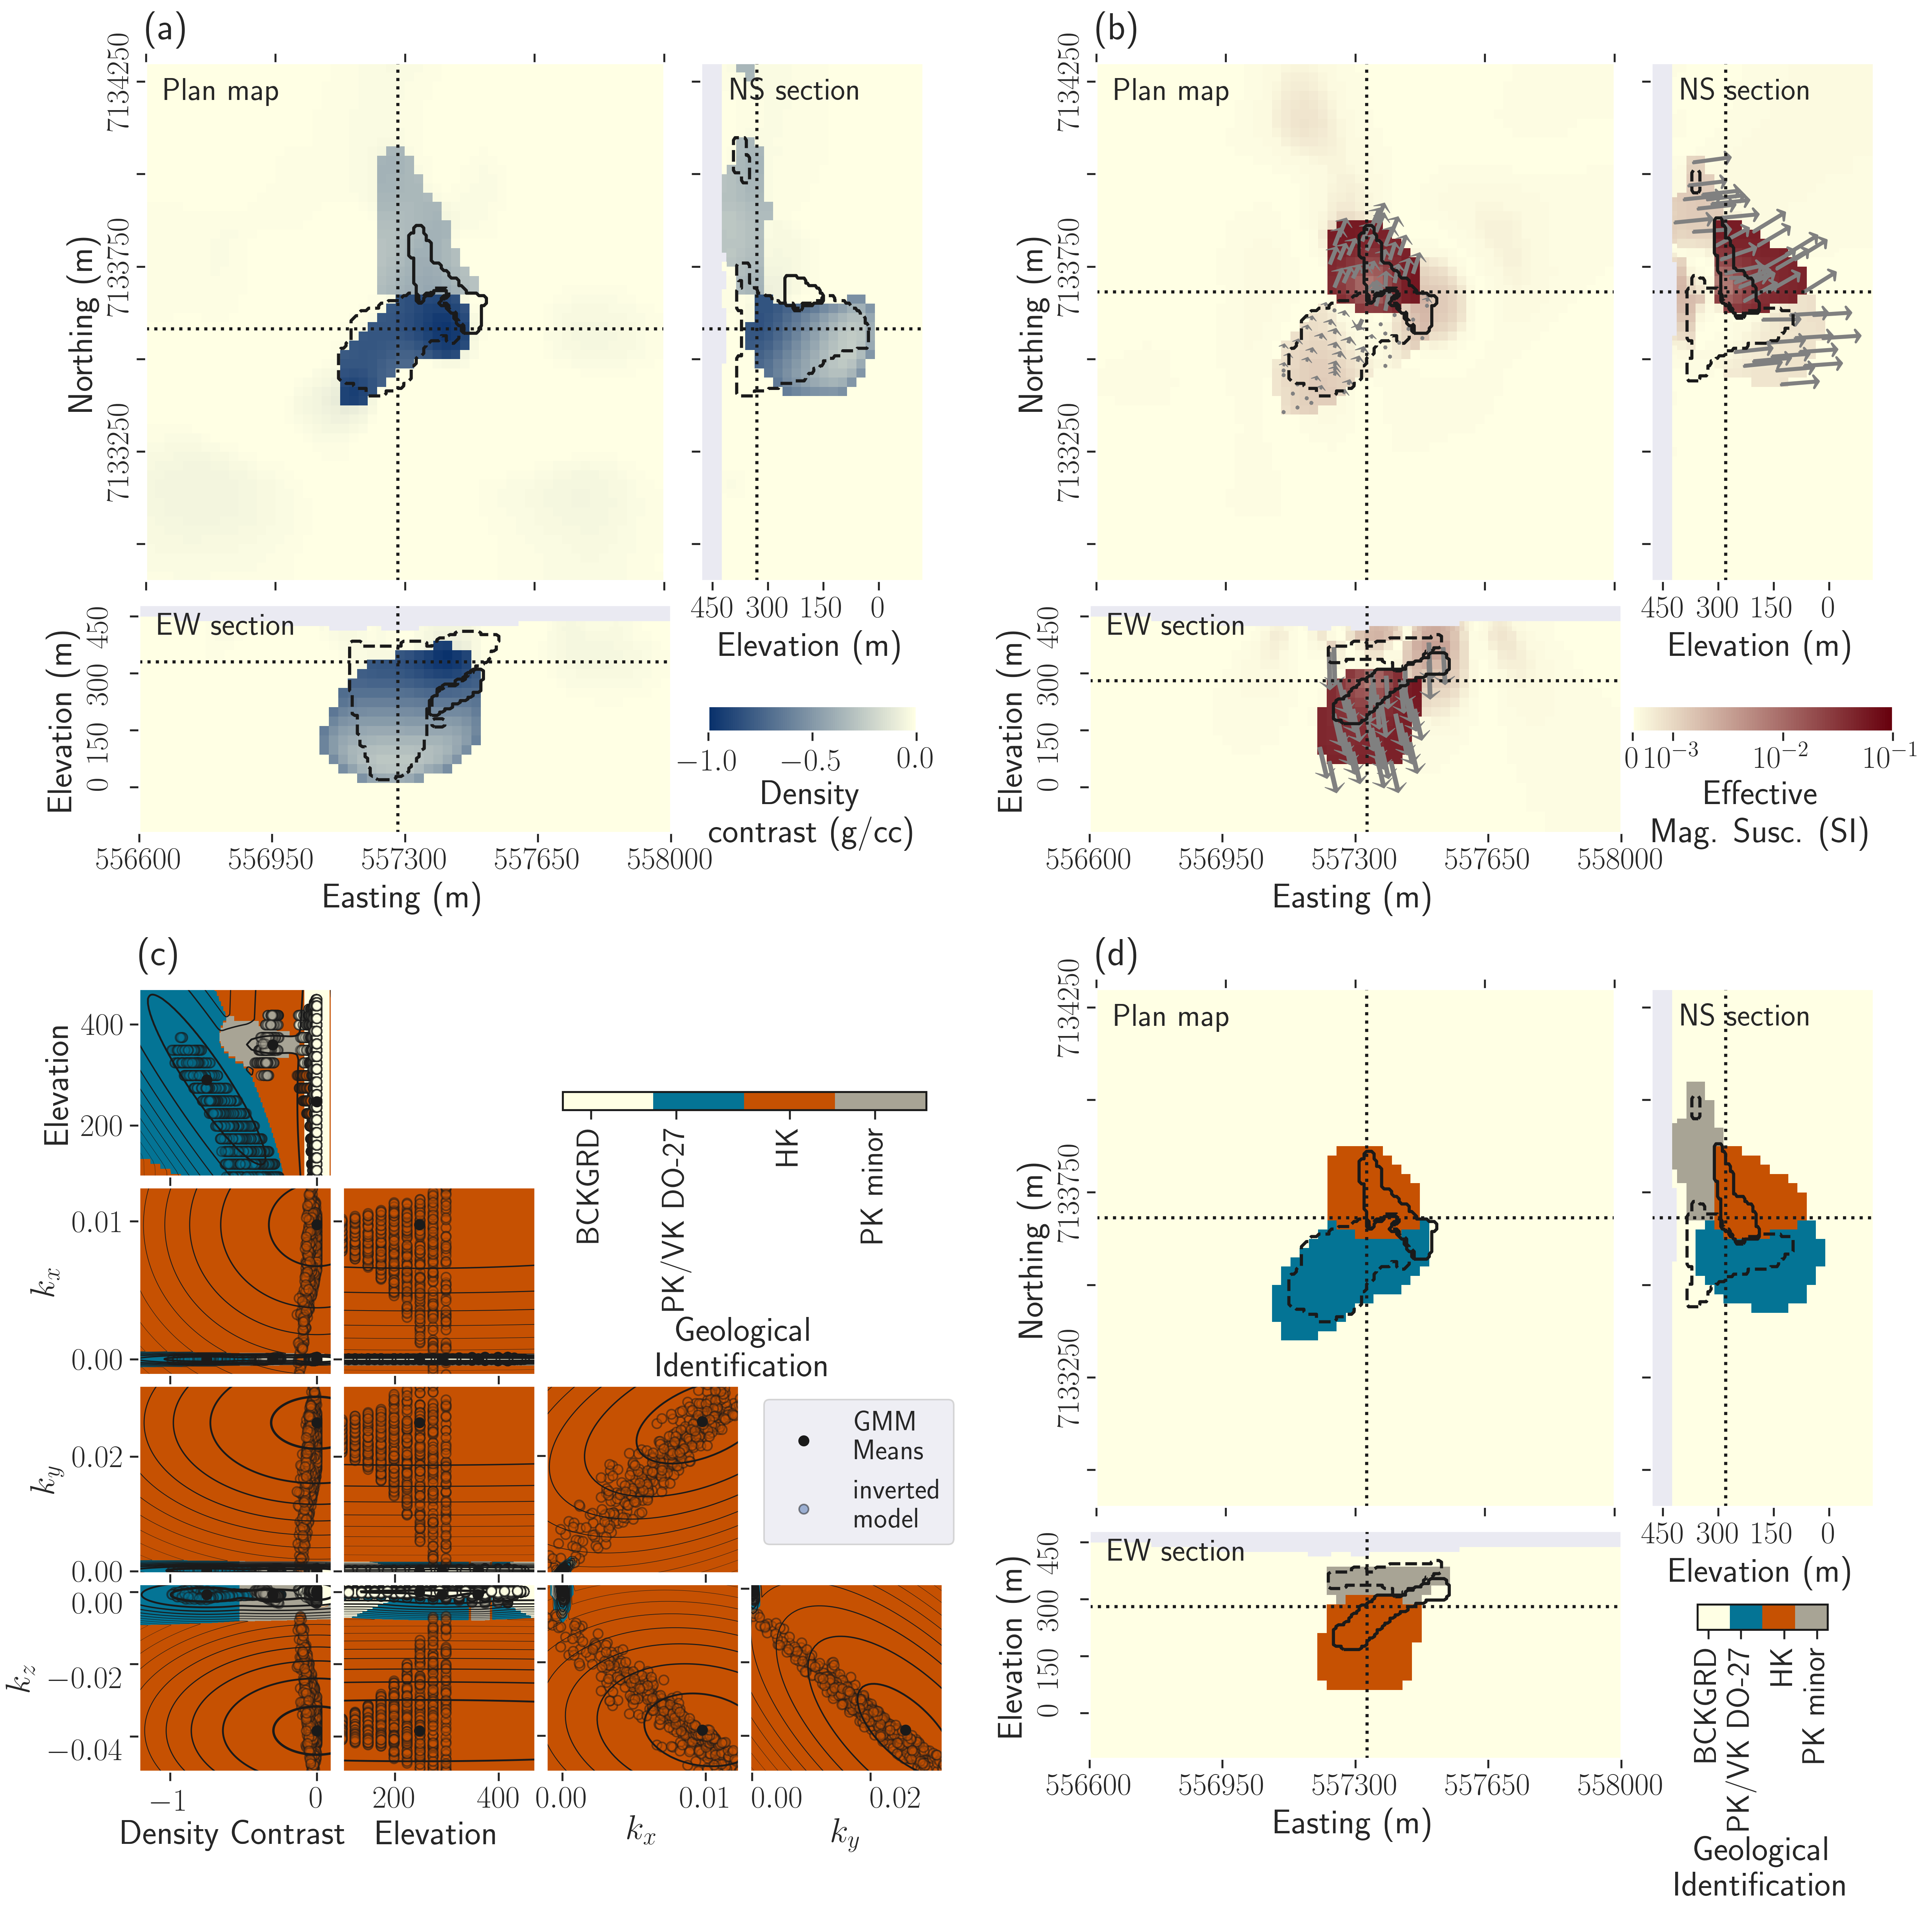
\includegraphics[width=\textwidth]{Figures/300dpi/Figure13.png}
\caption{Results of the multi-physics PGI with an additional rock unit for near-surface PK-minor occurrences, and geological domains. (a) Plan map, East-West, and North-South cross-sections through the density contrast model; (b) Magnetic vector model. The gray arrows are the projections of the magnetization directions (unit vector) on the plane for the kimberlite units; (c) Presentation of the $5$-dimensional GMM: visualization of all possible $2$D projections. Comparison with the recovered model represented as the scatter plots of the four physical properties of the geophysical model and the elevation; (d) Resulting quasi-geologic model from the multi-physics PGI with four rock units.}
\label{fig:Figure13.png}
\end{figure*}%*

%The geophysical surveys are individually fit, as well as the GMM petrophysical distribution. The normalized misfit maps are presented in Figure \ref{fig:Figure14.png}. The maps associated with gravity data are random and consistent with the assigned noise levels (Figures \ref{fig:Figure14.png}b to \ref{fig:Figure14.png}d). The misfits of the airborne gravity gradiometry data (Figures \ref{fig:Figure14.png}c and \ref{fig:Figure14.png}d) appear to follow the flight path. The flight lines were also visible in the data (Figure \ref{fig:Figure3.png}c and \ref{fig:Figure3.png}d). %It indicates the inversion successfully accounts for the uneven flight path across lines.
%For the magnetic data, even though we achieved the global geophysical target misfit, there is a coherent residual signal visible in the misfit map (Figure \ref{fig:Figure14.png}a). The misfits are higher, up to $7$ nT, just above the eastern extension of the HK body that we seem to not recover in the inversion (Figures \ref{fig:Figure12.png}b and \ref{fig:Figure12.png}d).

The result of the multi-physics inversion with an additional rock unit for near-surface kimberlites and geological domains is shown in Figure \ref{fig:Figure13.png}. This model is geologically appealing. It reproduces known geological features better than in the previous multi-physics inversion. The northern extension of the PK/VK pipe unit is now gone, and the general outline of the pipe is thus much better recovered. Most of the northern tip gravity anomaly is explained by a near-surface sheet of PK-minor units, whose locations match with known occurrences in drillholes. For the HK unit, we start to obtain some sense of the dip of that unit. Its near-surface outline is again well recovered, but its thickness appears overestimated.

The introduction of the new unit has also changed how well petrophysical signatures are recovered. The density contrast of the HK unit is now closer to the null density contrast measured in samples, at an average of $-0.03 \text{ g/cm}^3$ (compared to $-0.12 \text{ g/cm}^3$ in the previous multi-physics inversion with three rock units). Similarly, the PK/VK pipe unit is now very close to its measured magnetic amplitude at $8\cdot 10^{-4}$ SI (compared to $1.06 \cdot 10^{-3}$ SI in the previous multi-physics inversion). The orientations of the magnetization are also consistent with the values in the GMM: they align with the Earth's magnetic field for PK/VK-pipe and PK-minor and are along the remanence direction for the HK unit. The clustering of the magnetic petrophysical values of the HK unit is not as good as in previous inversions, but they are still within acceptable bounds as defined by its distribution.

%\plot{Figure14.png}{width=\textwidth}{Normalized data misfits for all the datasets from the multi-physics PGI with geological domains and four rock units. (a) For the magnetic data; (b) for the gravity data; (c) and (d) for the gravity gradiometry data.}


\begin{figure*}[!ht]
\centering
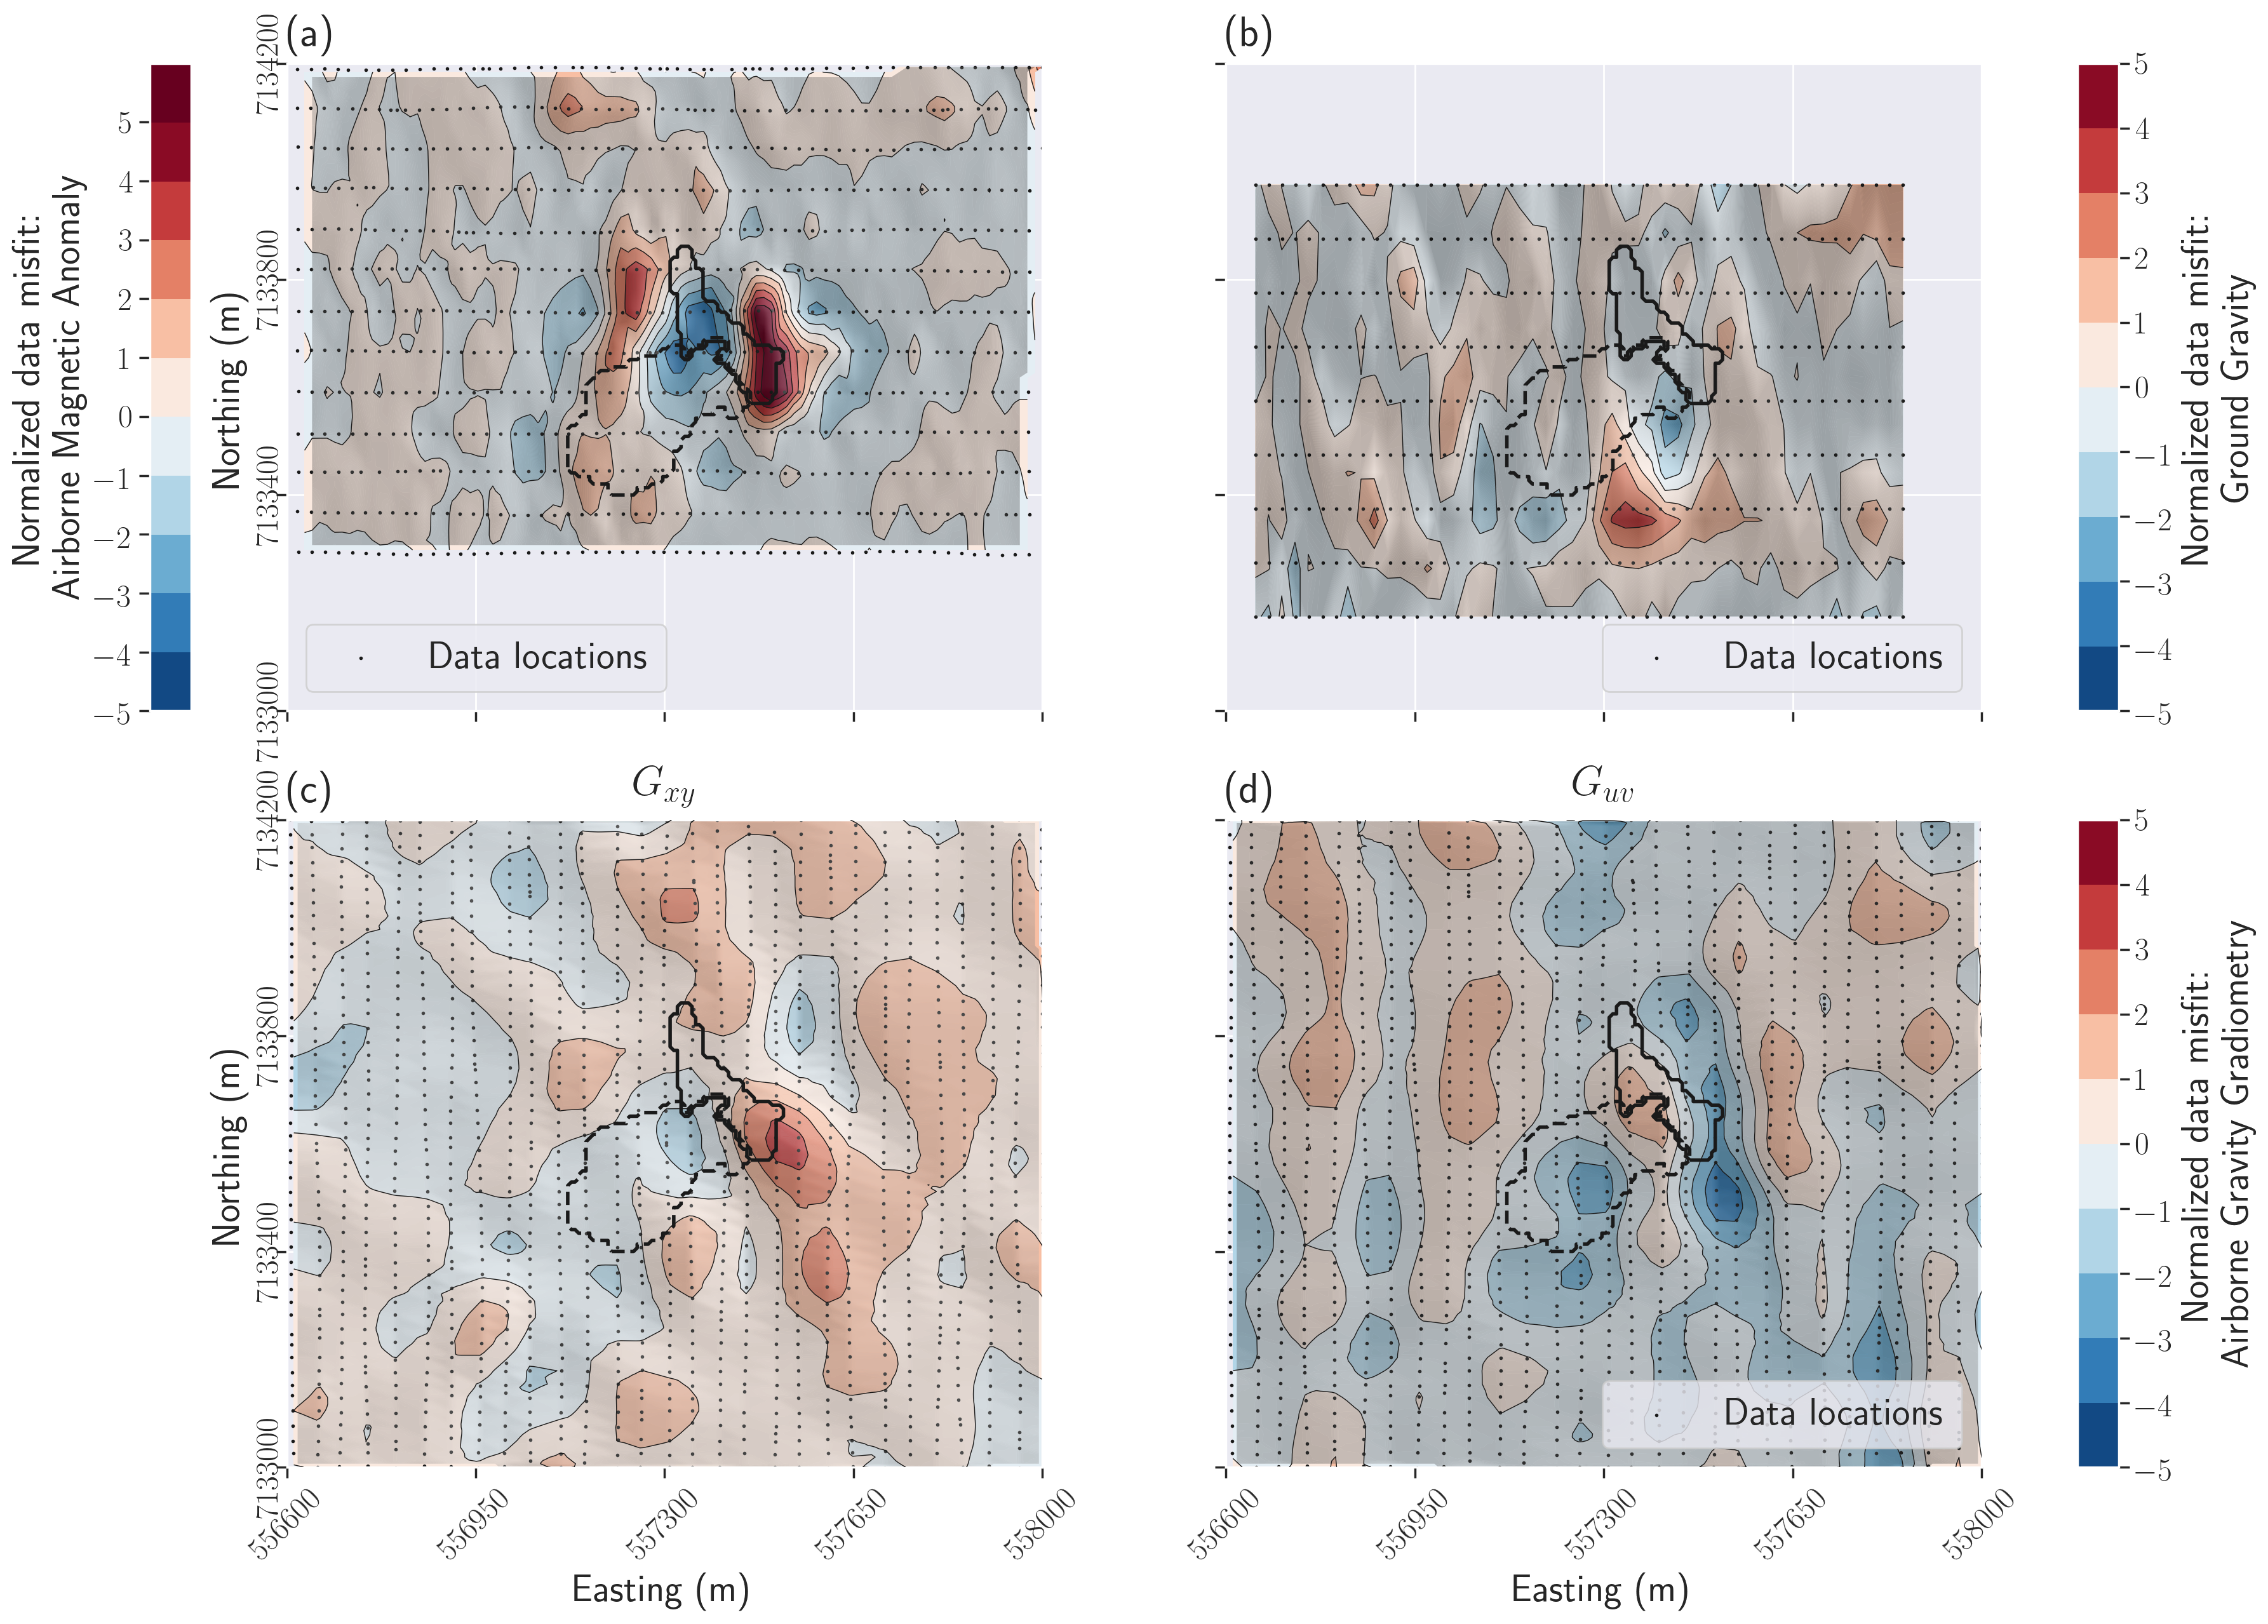
\includegraphics[width=\textwidth]{Figures/300dpi/Figure14.png}
\caption{Normalized data misfits for all the datasets from the multi-physics PGI with geological domains and four rock units. (a) For the magnetic data; (b) for the gravity data; (c) and (d) for the gravity gradiometry data.}
\label{fig:Figure14.png}
\end{figure*}

The geophysical surveys are individually fit, as well as the GMM petrophysical distribution. The data misfit value of each survey, divided by its number of data, is $0.99$ for the ground gravity survey, $0.84$ for the airborne gravity gradiometry survey, and $0.92$ for the airborne magnetic survey (targets of unity). The normalized data misfit maps are presented in Figure \ref{fig:Figure14.png}. The maps associated with gravity data are random and consistent with the assigned noise levels (Figures \ref{fig:Figure14.png}b to \ref{fig:Figure14.png}d). The misfits of the airborne gravity gradiometry data (Figures \ref{fig:Figure14.png}c and \ref{fig:Figure14.png}d) appear to follow the flight path. The flight lines were also visible in the observed data (Figure \ref{fig:Figure3.png}c and \ref{fig:Figure3.png}d). For the magnetic data, even though we achieved the global geophysical target misfit, there is a coherent residual signal visible in the misfit maps (Figure \ref{fig:Figure14.png}a). The misfits are higher, up to $7$ nT, just above the eastern extension of the HK body that we seem to not recover in the inversion (Figures \ref{fig:Figure12.png}b and \ref{fig:Figure12.png}d).

%It indicates the inversion successfully accounts for the uneven flight path across lines.

%______________________________________________________________________________
\section{Discussion}

The PGI framework has enabled us to jointly invert three types of geophysical data (airborne magnetic, ground gravity, and airborne gravity gradiometry) using five coupled parameters (density, elevation, and the three components of the magnetic vector). This joint approach recovers a final quasi-geologic model that maps all expected geological units (background, PK/VK pipe, HK, and PK-minor units) by reproducing their petrophysical characteristics in the inversion. This result is unobtainable by inverting datasets separately and then carrying out a post-inversion classification of the recovered physical properties.

%Post-inversion classification produces volumes of rocks with erroneous physical properties characteristics. These erroneous units can be avoided by fitting all the available datasets (geophysical or petrophysical) within a single inversion.

For this study, we have drillhole information, and we built a geologic model from it to compare with our results. For DO-$27$, the PK unit is the diamondiferous kimberlite unit and so estimating its volume and shape is key for resource estimation. While PK is indistinguishable from VK from the potential fields data, VK has a negligible volume in the geologic model compared to PK. We can, therefore, interpret the PK/VK-pipe unit as representing the diamondiferous PK unit. Reproducing the PK density signature, with its depth dependence, allows us to obtain an informed estimation of its shape and volume. The surface outline and bottom extension of the potentially diamondiferous unit are in good agreement with the geologic model, but the quasi-geologic model is more rounded at depth. The estimated volume of the PK/VK-pipe is evaluated at $28\cdot 10^6~\text{m}^3$ and can be compared to $15.7\cdot 10^6~\text{m}^3$, obtained from the geologic model (see \citet{HARDER2009} and Figure \ref{fig:Figure12.png}d). Most of the volume discrepancy is concentrated at depth, where the gravity surveys are less sensitive.

%The discrepancy is due to the northern extension of the pipe seen in the geophysical model. The geologic model does not have this extension, and drillholes in the area have not encountered any PK/VK unit below HK. However, gravity data, evaluated from forward modeling the DO-$27$ geologic model, underestimate the true gravity anomaly in the north and central portions of the map (Figure \ref{fig:TKC_DensityPredicted.png}). The missing volume of kimberlite from the geologic model requires to explain the gravity data is quite important. We did not succeed in explaining that discrepancy by lowering the assumed density of HK (within the range measured by the samples). A more detailed study of the density of the HK unit and minor near-surface kimberlite units would help further resolve that question.

From a numerical perspective, the MVI problem with petrophysical information has been more challenging than the gravity inversions. This is due in part to the orders of magnitude difference between the various units, the challenge of inverting for logarithmically distributed effective susceptibilities, and the lack of oriented samples to determine the magnetic characteristics of the HK unit. In principle, the use of MVI in spherical coordinates seems desirable, but the additional nonlinear transformations complicate an already challenging problem. We, therefore, implemented the Cartesian formulation. Nevertheless, we were still able to recover a unit with the identified magnetic signature of HK. Realistically, however, the geology is probably more complicated than we have modeled. Assuming a single and relatively uniform HK unit is likely insufficient to explain the whole magnetic data, as it is shown by the data misfit map in Figure \ref{fig:Figure14.png}a. During our study, we tried to obtain various estimates of the orientation of the remanent field, such as using a sparse MVI code in spherical coordinates \citep{SparseNorms2} or obtaining the best-fitting amplitude and angles for the available shape of HK in the geologic model. While the recovered inclinations appeared consistent across estimations with the value obtained in \citet{TKCpaper}, the declinations spanned a wide range. Those challenges could be explored in a future case study. While the inversion results seem to validate the current petrophysical estimates, the estimation of the density, magnetic susceptibility, and remanent magnetization orientation of the HK unit could be significantly improved by measuring new, oriented samples.

%The linear Cartesian formulation also appeared simpler to use than the nonlinear spherical formulation, for equivalent expected outcomes as we provide the PGI with petrophysical distributions to reproduce.
%We did use a spherical formulation during our experiments. But, Also, as we provide the PGI with petrophysical distributions to reproduce, the linear Cartesian formulation appeared simpler to use than the nonlinear spherical formulation, for equivalent expected outcomes.
%Another way would be to include the borehole lithology information directly into the inversion through the use of local proportions in the GMM \citep{ggz389}. None of the previous papers \citep{TKCpaper,TKCEM,TKCIP} use any sort of borehole information in the inversions. In this paper, we used petrophysical information, but we have not spatially constrained the construction of the quasi-geologic model by the location of the lithologies, such as observed in drillholes. It may improve the current geophysical data misfit map by guiding the inversion towards reproducing the borehole lithology. This approach could help resolve the discrepancy of the dipping and eastern extension of the HK unit between the geophysical inversion and the geologic model.

Finally, while we used local proportions to implement elementary geological expectations, a complete inclusion of all the drillhole information is yet to be done. It could help further refine the quasi-geologic model, such as narrowing the PK/VK pipe unit at depth or constraining the thickness of the HK unit. The inclusion and extrapolation of drillhole information within the PGI framework is part of our current research.

%______________________________________________________________________________
\section{Conclusion}

Inferences from inversions of single datasets, even when they are input into post-inversion classification algorithms, can be deficient. This limitation is a motivation to carry out joint inversions. The challenge is how to link the datasets together, in a practical sense, and how to include other relevant information. We adopt the PGI framework to use petrophysical measurements as the linkage and apply it to the field data acquired over the DO-$27$ kimberlite pipe. We have successfully jointly inverted airborne gradiometry, ground gravity, and airborne magnetic data, along with measured physical properties and geological information. Our framework outputs both physical property models and a quasi-geologic model. The results that include multiple physics, coupled with petrophysical and geological information, are shown to better resolve and distinguish the rock unit bodies compared to interpreting single-physics inversion results. The fact that we have been able to fit all the geophysical datasets while reproducing the petrophysical signatures, such as varying densities with depth and magnetization orientations, is a significant achievement.
%The quasi-geologic model successfully recovers the location and main structural features of the PK/VK and HK kimberlite pipe units. A third near-surface kimberlite facies, with distinct petrophysical properties inferred from inversions, is also imaged.
Working with a complex geologic model presents challenges, and the flexibility of the PGI framework offers multiple ways to tackle them. Refining the classification of rock units, testing for various petrophysical signatures, and defining local geological information to satisfy field observations have been keys to recover a satisfying quasi-geological model. Nevertheless, further refinements of our PGI implementation could improve the estimate of the volumes and structures of the PK and HK units. Such refinements could include a more extensive integration of the drillhole information, and address the complexity of the magnetization signatures. Moreover, there are other geophysical datasets that can provide constraints on the electromagnetic properties of the rock units, and incorporating those can further reduce the discrepancies between our geophysical and geologic models. The DO-$27$ kimberlite pipe presents an ideal test site on which to test these procedures.

%______________________________________________________________________________
\section{Acknowledgments}

The authors thank K. Witherly and J. Jansen for the inspiring discussions about the DO-$18$/DO-$27$ datasets over the past 15 years. We would also like to thank R. Enkin and D. Cowan for the insightful conversations about the measurements of petrophysical properties. We sincerely thank Condor Consulting Inc., Peregrine Diamonds Ltd., and Kennecott for making the datasets available for our research. Finally, we want to acknowledge the work of the \texttt{SimPEG} community \citep{Cockett2015}, without which this study would not have been possible, and especially L.J. Heagy for the development of tools to mix and add together objective-functions and J. Capriotti for the development of a fast Octree Mesh.

%\append{Gaussian parameters and Gaussian mixture model formulas}

%Let's consider a given petrophysical dataset with $n$ samples, denoted $\{\mathbf{x}_i,i=1..n\}$. Each $\mathbf{x}_i$ represents the various measured physical properties for the sample $i$. For each sample we know its current geological classification. This is denoted by $j=1..c$ where $c$ the number of distinct geological units. A sample $i$ belonging to unit $j$ is noted $\mathbf{x}_{i\in j}$. With known labels, the Gaussian distribution parameters for each unit $j=\{1..c\}$ are given in equations \ref{MLE-weights} to \ref{MLE-cov} (respectively its mean $\mathbf{\mu}_j$, its covariance matrix $\Sigma_j$, plus its relative proportion $\pi_j$).


%\begin{align}
%\pi_j &= \frac{n_j}{n}
%\label{MLE-weights}
%\end{align}

%\begin{align}
%\mathbf{\mu}_j &= \frac{1}{n_j}\sum_{i=1}^{n_j}\mathbf{x}_{i \in j}
%\label{MLE-means}
%\end{align}

%\begin{align}
%\Sigma_j & = \frac{1}{n_j}\sum_{i=1}^{n_j}(\mathbf{x}_{i \in j}-\mathbf{\mu}_j)(\mathbf{x}_{i \in j}-\mathbf{\mu}_j)^T.
%\label{MLE-cov}
%\end{align}

%Given the petrophysical signature of all known units, the probability function to observe an unlabeled physical property data point $\mathbf{x}_i$ can be written as a Gaussian Mixture Model (GMM) (see also Figure \ref{fig:Figure6.png}):

%\begin{align}
%&\mathcal{P}(\mathbf{x}_i|\Theta) = \sum_{j=1}^c \pi_j \mathcal{N}(\mathbf{x}_i|\mathbf{\mu}_j,\Sigma_j) \label{GMM}
%\end{align}

%The symbol $\mathcal{N}$ represents the Gaussian distribution function. The variable $\Theta$ holds the GMM parameters $\Theta= \left\{\pi_j, \mathbf{\mu}_j, \Sigma_j\right\}_{j=1..c}$.

%The geological identification is denoted $\mathbf{z}$. Given an unlabeled data point $\mathbf{x}_0$, its geological identification $z_0$ takes the value of the geological unit with the highest probability (see equation \ref{MAP_z_physProp}).

%\begin{align}
%&z_0 = \mathop{\hbox{argmax}}\limits_{z \in \left\{1..j\right\}}\mathcal{P}(\mathbf{x}_0|z)\mathcal{P}(z) \label{MAP_z_physProp}\\
%&\text{with:} \nonumber \\
%&\mathcal{P}(z) = \pi_z \text{ and}\label{weight_z_prior} \\
%&\mathcal{P}(\mathbf{x}_0|z)=\mathcal{N}(\mathbf{x}_0| \mathbf{\mu}_{z},\Sigma_{z}).
%\end{align}

%\append{HK density samples}

%\tabl{hktable}{HK density samples.}{
%\begin{center}
%\scalebox{0.9}{
%\begin{tabular}{|c|c|}
%\hline
%Sample number & Density \\
%\hline
%\#1 & 2.764 \\
%\#2 & 2.867 \\
%\#3 & 2.435 \\
%\#4 & 2.632 \\
%\#5 & 2.677 \\
%Mean Value & 2.675 \\
%\hline
%\end{tabular}}
%\end{center}
%}
%\append{coupling GMM parameters}


\bibliographystyle{seg} % style file is seg. bst
\bibliography{biblio}

\end{document}
